\documentclass[titlepage]{article}

\usepackage[utf8]{inputenc}
\usepackage{fullpage}
\usepackage{enumitem}
\usepackage{fixltx2e}
\usepackage{amsmath}
\numberwithin{equation}{section}
\usepackage[dutch]{babel}
\usepackage[colorinlistoftodos]{todonotes}
\usepackage{float}
\restylefloat{table}
\restylefloat{figure}
\setlist[enumerate]{label*=\arabic*.}
\usepackage{graphicx}
\usepackage{pdfpages}
\usepackage{fourier}
\graphicspath{ {images/} }

\begin{document}

%voorblad toevoegen aan hoofdbestand
\begin{titlepage} 
\newcommand{\HRule}{\rule{\linewidth}{0.5mm}} 
\center 
\textsc{\LARGE KU Leuven}\\[1.5cm] 
\textsc{\Large Informatica}\\[0.5cm] 
\textsc{\large Statiestiek en Data-analyse}\\[0.5cm]
\HRule \\[0.4cm]
{ \huge \bfseries Samenvatting}\\[0.4cm]\HRule \\[1.5cm]
\Large \emph{Autheur:}\\
Kevin \textsc{Coorens}\\[3cm]
{\large \today}\\[2cm] 
\vfill

\end{titlepage}

%leeg blad achterkant voorblad
\thispagestyle{empty}
\clearpage\mbox{}\clearpage

%romeinse paginanummering starten voor inhoudstafel
 \pagenumbering{roman}
\tableofcontents
\newpage
%arabische nummering starten voor de rest van het document
 \pagenumbering{arabic}
 
\section{Doel van de statistiek}
\subsection{Inleiding}
\subsection{Verzamelen van gegevens}
\textbf{Variabelen} 
\begin{itemize}
  \item eigenschappen die gemeten worden
  \item genoteerd met hoofdletters
  \item afgekort met kleine letter p
\end{itemize}
\textbf{Steekproefgrootte}
\begin{itemize}
  \item aantal metingen die verricht worden
  \item genoteerd met kleine letter n
\end{itemize}
\subsection{Classificatie van gegevens}
\subsubsection{Kwalitatieve en kwantitatieve gegevens}
\textbf{Nominale meetniveau}
\begin{itemize}
  \item gebruikt om onderzoekseenheden te klasseren
  \item niet te interpreteren in termen van meer of minder $(<,>)$
  \item wel gebruikt om na te gaan of elementen al dan niet gelijk zijn.
\end{itemize}
\textbf{Ordinale meetniveau}
\begin{itemize}
	\item elementen kunnen geordend worden via een bepaald ordeningscriterium
	\item schaal is geijkt
\end{itemize}
\textbf{Metrische meetniveau}
\begin{itemize}
	\item gegevens sluiten meer aan bij meten
	\item uitgedrukt in hoeveelheden
	\item meer of minden kan uitgedrukt worden, maar ook hoeveel meer of minder
\end{itemize}
\subsubsection{Discrete en continue gegevens}
\textbf{Discrete gegevens}
\begin{itemize}
	\item tussen twee willekeurige elementen kan geen derde element bijgedacht worden
	\item aantal elementen van de uitkomstverzameling is eindig
\end{itemize}
\textbf{Continue gegevens}
\begin{itemize}
	\item tussen twee willekeurige elementen kan een derde element bijgedacht worden
	\item aantal elementen van de uitkomstverzameling is oneindig
\end{itemize}
\subsection{Van steekproef naar populatie}
\textbf{Steekproefgemiddelde}
\begin{itemize}
	\item het gemiddelde over alle bekomen waardes van de steekproef
	\item is slechts een benadering, mag niet veralgemeend worden, bij nieuwe steekproef waarschijnlijk ook nieuw steekproefgemiddelde
\end{itemize}
\textbf{Wet van grote aantallen}
\begin{itemize}
	\item volgens welke steekproefeigenschappen de eigenschappen van een oneindige verzameling dichter naderen, naarmate de steekproef groter wordt
\end{itemize}
\subsection{Samenvatting}
\begin{itemize}
	\item De populatie is het geheel van objecten of mensen waarover men een beslissing wil nemen. Eén zo'n object of persoon is een onderzoekseenheid
	\item De verschillende kenmerken gemeten voor die objecten of mensen worden variabelen genoemd.
	\item De uitkomstenverzameling is de verzameling van alle mogelijke uitkomsten voor een variabele. Deze verzameling wordt afgekort als $\ell$.
	\item In de praktijk worden er slechts metingen gedaan voor een steekproef of een kleine groep van n objecten. Hierbij wordt n de steekproefgrootte of steekproefomvang genoemd. Voor elke variabele zijn er dus n metingen die als volgt genoteerd kunnen worden: $x_{1}$, ..., $x_{n}$.
	\item De metingen van verschillende variabelen worden samengevoegd in de kolommen van een gegevensmatrix.
	\item Afhankelijk van deze uitkomstenverzameling $\ell$ zijn er verschillende types van gegevens. Een opdeling kan worden gemaakt op basis van het meetniveau van de uitkomsten: kwalitatief of kwantitatief. De kwalitatieve gegevens kunnen opgesplitst worden in nominale en ordinale gegevens. Gegevens kan men ook onderscheiden op basis van de omvang van de uitkomstenverzameling. Bij discrete gegevens is de uitkomstenverzameling eindig of aftelbaar oneindig, terwijl deze bij continue gegevens oneindig groot is.
	\item Om bij het nemen van beslissingen de stap van steekproef naar populatie te zetten is de wet van grote aantallen essentieel.
\end{itemize}
\subsection{Gegevens uit verschillende onderzoeksdomeinen}
Voor voorbeelden zie handboek blz. 18 t.e.m. blz. 28.
\section{Beschrijvende statistiek}
\subsection{Absolute en relatieve frequenties}
\subsubsection{Staafdiagram voor een kwalitatieve variabele}
\textbf{Absolute frequentie}
\begin{itemize}
	\item voor elke mogelijke uitkomst m\textsubscript{j} uit de uitkomstverzameling het aantal uitkomsten x\textsubscript{i} in de steekproef tellen die gelijk zijn aan m\textsubscript{j}
	\item voorstelling $\rightarrow$ staafdiagram
\end{itemize}
\newpage
\textbf{Relatieve frequentie}
\begin{itemize}
	\item nodig om frequentiegegevens op eenzelfde schaal te zetten
	\item soms ook wel steekproefproporties genoemd
	\item $\sum\limits_{j=1}^k f\textsubscript{j,n} = \frac{n_{1}}{n}+\frac{n_{2}}{n}+...+\frac{n_{k}}{n}$
	\item voorstelling $\rightarrow$ taartdiagram
\end{itemize}
\subsubsection{Histogram voor een kwantitatieve variabele}
\textbf{Discretisatie of groepering van de gegevens}
\begin{itemize}
	\item men deeelt de oplossingsverzameling op in een eindig aantal aangrenzende deelintervallen of klassen
	\item meestal alle klassen van gelijke breedte $\rightarrow$ klassenbreedte, $\Delta$ genoteerd
	\item voorstelling $\rightarrow$ histogram
	\item klassen bepalen? Niet te veel klassen (te gepiekt histogram), niet te weinig klassen (te sterk uitgevlakt histogram)
	\item regel voor bepalen van aantal klassen $\rightarrow$ formule van Sturges: \newline aantal klassen $= [log_{2}(n)+1]$ waarbij $[x]$ het kleinste gehele getal is dat niet kleiner is dan x
\end{itemize}
\textbf{Histogram met frequentiedichtheden}
\begin{itemize}
	\item hoogte van een balk boven een klasse is gelijk aan de relatieve frequentie van die klasse gedeeld door de overeenkomstige klassenbreedte 
	\item $h_{j}$ = $h(m_{j})$ = $\frac{f_{j,n}}{\Delta_{j}}$ = $\frac{n_{j}}{\Delta_{j}n}$
	\item oppervlakte van balken en dus niet hoogte, geeft aan hoe vaak bepaalde uitkomsten voorkomen
\end{itemize}
\subsection{Vormen van verdelingen}
\subsubsection{Symmetrische verdelingen}
\begin{itemize}
	\item gedragen zich op dezelfde wijze aan de linkse en rechtse zijde van de figuur
	\item Het histogram gaat over zichzelf indien men de figuur horizontaal spiegelt om het midden
	\item in de praktijk komt perfecte symmetrie nagenoeg nooit voor, we moeten ons dus tevreden stellen met een benaderende symmetrie
\end{itemize}
\subsubsection{Normale verdelingsvorm}
\begin{itemize}
	\item ook wel Gaussische veredeling genoemd
	\item duidelijk maximum in het midden van de figuur
	\item langs beide zeiden van de top neemt de verdeling in stapjes af
	\item naarmate de steekproefgrootte toeneemt, begint het histogram meer en meer op een klokcurve te lijken
\end{itemize}
\subsubsection{Andere verdelingsvormen}
\textbf{Scheve (niet-symmetrische) verdelingen}
\begin{itemize}
	\item verdeling die aan één zeide trager neervalt of afzwakt dan aan de andere zeide
	\item rechtsscheve verdeling $\rightarrow$ rechter-staart zwakt trager af dan linker-staart
	\item linksscheve verdeling $\rightarrow$ linker-staart zwakt trager af dan rechter-staart
\end{itemize}
\begin{flushleft}
\textbf{Verdelingen met zware (of lange) staarten}	
\end{flushleft}
\begin{itemize}
	\item symmetrisch maar toch niet normaal
	\item staarten vallen trager naar nul dan bij de klokvorm van de normale verdeling
\end{itemize}
\textbf{Verdelingen met lichte (of korte} staarten
\begin{itemize}
	\item histogrammen waarbij we moeilijk over een staart kunnen spreken (zie voorbeeld met de dobbelstenen)
\end{itemize}
\textbf{Bimodale verdelingen}
\begin{itemize}
	\item histogrammen met twee (of eventueel meer) doelgroepen en dus ook toppen
\end{itemize}
\textbf{Uitschieters}
\begin{itemize}
	\item Soms hoort één of een relatief klein aantal getallen niet echt bij de rest van de gegevensgroep
	\item meestal gaat men trachten te achterhalen waarom de gevonden uitschieters zo verschillend zijn (tikfout, extra gunstige/ongunstige omstandigheden)
\end{itemize}
\subsection{Cumulatieve frequenties en kwantielen}
\subsubsection{Cumulatieve verdelingsfunctie}
\textbf{Algemeen} $\rightarrow$ cumulatieve verdelingsfunctie in een waarde x is gelijk aan het relatief aantal steekproefuitkomsten $x_{i}$ die niet groter zijn dan x
\begin{center}
	$\hat{F}_{n}$($x$) = $\frac{1}{n}$ (aantal $x_{i}$ $\leq$ $x; i = 1, ...,n$)
\end{center}
Kan berekend worden in elke reële waarde, niet enkel in de steekproefuitkomsten.
\subsubsection{Kwantielfunctie}
Dit is het omgekeerde van de cumulatieve verdelingsfunctie, gegeven een bepaald percentage, welk reëel getal situeert zich dan in de overeenkomstige positie in de steekproef? We gaan dus de inverse functie van de cumulatieve verdelingsfunctie proberen te bepalen. (dit kan echter niet zomaar wegens de trapfunctie)\newline
\newline\textbf{Algemeen} $\rightarrow$ $\hat{Q}_{n}(p)$ is het kleinste getal $x$ waarvoor $\hat{F}_{n}$($x$) $\geq p$\newline \newline
De kwantielen $\hat{Q}_{n}(0.25)$, $\hat{Q}_{n}(0.5)$ en $\hat{Q}_{n}(0.75)$ worden vaak beschouwd en hebben daarom een aparte naam gekregen. Ze worden respectievelijk het eerste, tweede en derde kwartiel genoemd.
\subsection{Centrumkenmerken}
\subsubsection{Steekproefgemiddelde}
\begin{equation}
	\bar{x} = \frac{1}{n}(x_{1} + ... + x_{n}) = \frac{1}{n} \sum\limits_{i=1}^n x_{i}
	\label{2.9}
\end{equation}
\begin{itemize}
	\item enkel voor metrische gegevens
	\item erg gevoelig voor uitschieters
\end{itemize}
\subsubsection{Mediaan}
\begin{equation}
	med(x_{1}, ... , x_{n} = \begin{cases} (x_{((n+1)/2)}, & \mbox{als } n\mbox{ oneven} \\ x_{(n/2)} + x_{((n/2)+1)})/2, & \mbox{als } n\mbox{ even} \end{cases}
	\label{2.10}
\end{equation}
\begin{itemize}
	\item geeft de middelste waarde van de geordende steekproef aan
	\item voor symmetrische verdelingen vaak ongeveer gelijk aan het steekproefgemiddelde
	\item het bestuderen van het verschil tussen het steekproefgemiddelde en de mediaan is daarom nuttig om een idee te vormen omtrent het al dan niet symmetrisch zijn van de verdelingsvorm
\end{itemize}
\subsubsection{Getrimd gemiddelde}
Een vast percentage (bv. 5 of 10 procent) van de kleinste en de grootste waarden wordt weggelaten uit de gegevensverzameling en men berekent nu het gemiddelde van de resterende gegevens. Nadeel hiervan is dat het trimpercentage gekozen moet worden zonder dat er te veel reguliere punten en te weinig uitschieters verwijdert worden.
\subsubsection{Modus}
De modus is (zo die bestaat en uniek is) het element uit de uitkomstenverzameling dat het meeste voorkomt in de tseekproef, of dat met andere woorden de hoogste frequentie vertoont. Bij een histogram gebaseerd op continue gegevens wordt de modus gedefineerd als het klassenmidden waar het gekozen histogram de hoogste waarde bereikt.
\subsection{Spreidingskenmerken}
\begin{center}
	$R = x_{(n)} - x_{(1)}$
\end{center}
\begin{itemize}
	\item geeft afstand weer tussen de grootste $x_{(n)}$ en de kleinste waarneming $x_{(1)}$
	\item erg afhankelijk van de steekproefgrootte
	\item erg gevoelig aan uitschieters
\end{itemize}
\subsubsection{Standaardafwijking en variantie}
Uitgaande van een zekere centrummaat kan men globale spreidingskenmerken verkrijgen door de afstand tussen elke meetwaarde $x_{i}$ en die centrummaat te bepalen en vervolgens een centrumkenmerk te beschouwen van al die afstanden. 
\newline\newline\textbf{Algemeen}
\begin{center}
	$s^ = \sqrt{\frac{1}{n - 1} \sum\limits_{i=1}^n (x_{i} - \bar{x})^2}$ 
\end{center}
\begin{center}
	$s^2 = \frac{1}{n - 1} \sum\limits_{i=1}^n (x_{i} - \bar{x})^2$ 
\end{center}
\textbf{Voor discrete waarden}
\begin{center}
$ s = \sqrt{\frac{1}{n - 1} \sum\limits_{j=1}^k (m_{j} - \bar{x})^2 n_{j}}$
\end{center}
\textbf{Hoe interpreteren}
Standaarddeviatie wordt gebruikt om mee te delen hoe exentrisch een observatie of steekproefwaarde is ten opzichte van het centrumkenmerk. 
\newline\newline Bij gegevens die uit een \textit{normale verdelin} voortkomen, geldt dat
\begin{itemize}
	\item steeds ongeveer twee derde van de gegevens binnen een afstand van één standaarddeviatie aan weerszijden van het steekproefgemiddelde ligt
	\item steeds ongeveer 95 procent van de gegevens binnen een afstand van twee standaarddeviaties aan weerzszijden het steekproefgemiddelde ligt.
\end{itemize}
De \textbf{z-score} is een equivalente manier om bovenstaande regels te formuleren
\begin{center}
	$z_{i} = \frac{x_{i} - \bar{x}}{s}$
\end{center}
\subsubsection{Interkwartielafstand}
\begin{itemize}
	\item minder gevoelig aan uitschieters
	\item geeft de lengte van een gebied weer rond de mediaan gelegen, dat ongeveer de helft van de gegevens omvat
\end{itemize}
\begin{center}
	$IQR = \hat{Q}_{n}(0.75)-\hat{Q}_{n}(0.25)$
\end{center}
Het is een algemene regel voor gegevens met een normale verdelingsvorm dat de verhouding tussen de IQR en de standaarddeviatie ongeveer een constante is.
\begin{center}
	$\frac{IQR}{s} \sim 1.34$
\end{center}
Men kan de waarde van IQR/s dus als een van de middelen hanteren om na te gaan of gegevens al dan niet uit een normale verdeling voortkomen.
\subsubsection{Median Absolute Deviation}
\begin{center}
$MAD = \underset{i=1, ... , n}{med} |x_{i} - med(x_{1}, ... , x_{n})|$
\end{center}
\begin{itemize}
	\item is de afstand van elke observatie tot de mediaan en dan de mediaan van al deze afstanden
	\item MAD is ongeveer de helft de IQR
	\item MAD/s $\sim$ 0.67
	\item kan tot 50 $\%$ uitschieters verdragen
\end{itemize}
\newpage
\subsection{Boxplot}
Om een beter idee te krijgen van de belangrijke kenmerken van een verdeling van steekproefelementen, zal men waarden zoals het gemiddelde, de mediaan, de kwartielen en kleinste en de grootste waarde op een schematische wijze proberen voor te stellen.
\begin{figure}[H]
\caption{Indeling van een boxplot}
	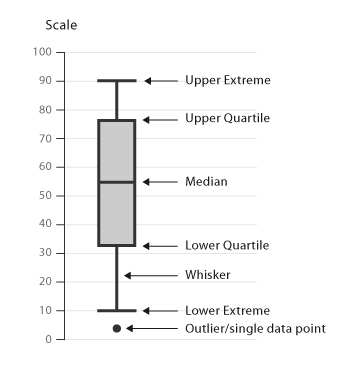
\includegraphics[scale=0.75]{images/boxplot}
\end{figure}
\textbf{Karakteristieken van een boxplot}\newline\newline
\textbf{Centrum:} De mediaan en eventueel het gimeddelde zijn als centrummaten aangeduid.\newline
\textbf{Spreiding:} De lengte van de doos stemt overeen met de interkwartielafstand IQR.\newline
\textbf{Scheefheid:} De positie van de mediaan ten opzichte van het eerste en het derde kwartiel geeft reeds aan of er asymmetrie is of niet. (bij rechtsscheve verdelingen ligt mediaan in onderste helft, bij linksscheve in bovenste helft) Rechtsscheve verdelingen geven aanleiding tot boxplots waarbij de bovenste whisker langer is dan de onderste. (net andersom voor linksscheve verdelingen)\newline
\textbf{Zwaarte van de staarten:} Indien veel mogelijke uitschieters aangeduid worden duid dit vaak op een zwaarstaartige verdeling. We mogen verwachten dat ongeveer 1\% van de gegevens
 toch als mogelijke uitschieter aangeduid worden. Vinden we er buidend meer, dan wijst dit op ofwel de aanwezigheid van echte uitschieters ofwel op een niet normale verdeling.\newline\newline
 \textbf{Nadeel} $\rightarrow$ deelgroepen aanwezig bij een bimodale verdeling zullen niet gedetecteerd worden. Maak dus ook steeds een histogram van de gegevens om een zo volledig mogelijk beeld te scheppen.\newline\newline
 \textbf{Merk op!} Een boxplot duidt uitschieters aan aan de hand van het eerste en derde kwantiel en de IQR. Deze kenmerken zijn minder gevoelig aan uitschieters dan het gemiddelde en standaardafwijking. Het is daarom ook niet verstandig om de z-score te gebruiken om uitschieters te detecteren!
 \subsection{Transformaties}
 Soms is het handig om metingen te transformeren zodat ze een meer symmetrische verdeling opleveren, dit wordt nu besproken in de volgende sectie.
 \subsubsection{Lineaire transformaties}
 \begin{center}
 	$g(x_{i}) = a + bx_{i}$ met $a,b \in {\rm I\!R}$
 \end{center}
 \textbf{Algemeen} $\rightarrow$ gegevens $x_{i}$ verschoven over een afstand $a$ en herschaald met een factor $b$.\newline\newline
 Voor de standaardafwijking s (en eveneens voor IQR en MAD) vinden we dat de waarde corresponderend met de nieuwe gegevens verkregen wordt door de maat berekend uit de oorspronkelijke gegevens te vermenigvuldigen met $|b|$.
 \begin{center}
 	$s_{g} = |b| s_{x}$ \ en dus \ $s_{g}^2 = b^2s_{x}^2$
 \end{center}
 Het verschuiven van de gegevens heeft dus geen effect op de spreidingsmaten.\newline\newline
 Een specifieke transformatie is die waarbij de metingen $x_{i}$ omgezet worden naar de $z$-scores. Dit kan bereikt worden door een transformatie met $a = - \frac{\bar{x}}{s_{x}}$ en $b = \frac{1}{s_{x}}$.\newline\newline
 \textbf{Opmerking} $\rightarrow$ Het gemiddelde van de $z$-scores is steeds gelijk aan 0 en hun variantie is steeds gelijk aan 1.
 \subsubsection{Monotoon stijgende transformaties}
 \begin{center}
 	$g(x) = a + bx$ \ waarbij \ $b>0$
 \end{center}
 Voorbeelden van monotoon stijgende transformaties zijn: de logaritmische functie, de exponentiële functie, de functies $x^2$ en $\sqrt{x}$ (voor $x > 0$).
 \subsection{Verbanden tussen twee variabelen}
 In de volgende sectie bestuderen we het verband tussen verschillende variabelen in een dataset. Een voorbeeld hiervan is, is het inkomensniveau afhankelijk van de regio?
 \subsubsection{Twee kwalitatieve variabelen}
 \begin{itemize}
 	\item kan worden weergegeven in een kruistabel
 	\item telt hoe vaak elke combinatie van twee variabelen in de steekproef voorkomt (absolute frequentie)
 	\item Uit de kruistabel die de frequenties voor de gezamenlijke uitkomsten weergeeft, kunnen we dus ook de frequenties voor de afzonderlijke variabelen berekenen.
 	\item staafdiagrammen vaak gebruikt voor een visuele voorstelling
 	\item telt hoe vaak elke combinatie van twee variabelen in de steekproef voorkomt en deelt dit dan door de totale steekproefomvang $n$ (relatieve frequenties)
 	\item vaak is men ook geïnteresseerd in voorwaardelijke frequenties, bijvoorbeeld men wil weten welk percentage van de steden in de Midwest inkomensniveau 1 heeft (men gaat hier dus enkels gegevens Midwest beschouwen)
 	\item voor voorwaardelijke frequenties gaat men in de tabel met absolute frequenties elke cel delen door het rijtotaal om zo een percentage te bekomen
 \end{itemize}
 \subsubsection{Een kwantitatieve en een kwalitatieve variabele}
 \begin{itemize}
 	\item kwalitatieve en kwantitatieve variabele met eindige uitkomstenverzameling $\rightarrow$ hanteer technieken uit vorige sectie
 	\item kwalitatieve en kwantitatieve variabele met oneindige uitkomstenverzameling $\rightarrow$ verdeling van de kwantitatieve variabelen voor de verschillende waarden van de kwalitatieve variabele naast of over elkaar uitzetten in een histogram, ook boxplots worden hiervoor gebruikt vooral voor meerdere groepen maakt dit het geheel overzichtelijker
 \end{itemize}
 \subsubsection{Twee kwantitatieve variabelen}
 Voor de visualisatie van het verband tussen twee kwantitatieve variabelen kunnen we gebruik maken van een histogram in drie dimensies (bivariate histogram). De variabelen worden opgedeeld in klassen en voor elke combinatie van klassen geven we weer hoe vaak die voorkomt aan de hand van frequenties.Op de verticale as kunnen uiteraard ook de relatieve frequenties aangeduid worden.\newline\newline
 Een andere voorstelling is een twee dimensionale voorstelling waar aan de hand van kleurtjes (donkere kleuren voor hoge frequentie en lichte kleuren voor een lage frequentie) zal aangegeven worden hoe hoog een balk is.
 \subsubsection{Covariantie en correlatiecoëfficiënt}
 Naast een histogram kunnen we ook andere tweedimensionale voorstellingen gebruiken voor metrische gegevens zoals bijvoorbeeld een \textit{puntenwolk} of \textit{spreidingsdiagram}. Op de horizontale as plotten we de meting voor de ene variabele en op de verticale as de meting voor de andere variabele.\newline\newline
 Indien een puntenwolk stijgt naar rechts spreekt men over een positieve associatie, daalt de puntenwolk dan spreken we van een negatieve associatie.\newline
 Uit de puntenwolk kunnen we ook de sterkte van de associatie aflezen, hoe dikker de wolk hoe sterker de associatie tussen de twee variabelen. Een sterke associatie tussen twee variabelen drukt uit dat de kennis van een van de variabelen de andere goed helpt voorspellen. (vice versa voor zwakke associaties)\newline\newline
 We willen nu de informatie over de associatie tussen twee variabelen X en Y meten, of weergeven in één getal. Hiervoor delen we de scatterplot (puntenwolk) op in vier kwadranten rond het punt met als coördinaten de steekproefgemiddeldes ($\bar{x}, \bar{y}$). In geval van een positieve associatie zal men uiteraard meer observaties terugvinden in de kwadranten linksonder en rechtsboven. Om dit in een getal uit te drukken voeren we de \textit{steekproefcovariantie}.
 \begin{center}
 	$s_{xy} = \frac{1}{n - 1}\sum\limits_{i=1}^n (x_{i} - \bar{x})(y_{i} - \bar{y})$
 \end{center}
 Algemeen geldt dat indien we de metingen $(x_{i}, y_{i})$ transformeren naar
 \begin{center}
 	$u_{i} = a_{1} + b_{1}x_{i}$ \ en \ $v_{i} = a_{2} + b_{2}y_{i}$
 \end{center}
 met $a_{1}, a_{2}$ en $b_{1}, b_{2}$ willekeurige reële getallen, dat
 \begin{center}
 	$s_{uv} = b_{1}b_{2}s_{xy}$
 \end{center}
 Op basis van de covarianties kunnen we dus niet beslissen of het om een sterke of zwakke associatie gaat. Hiervoor voeren we bijgevolg de \textit{(Pearson correlatiecoëfficiënt} $r_{xy}$ of kortweg $r$ in.
 \begin{center}
 	$r_{xy} = r = \frac{s_{xy}}{s_{x}s_{y}}$  
 \end{center}
 Dit geldt voor $s_{x}$ en $s_{y}$ groter dan nul. Merk ook op dat $s_{x} = 0$ (analoog voor $s_{y}$) zich enkel kan voordoen indien alle $x_{i}$ gelijk zijn!
 Men kan ook aantonen (boek blz. 86) dat voor de correlatiecoëfficiënt geldt dat:
 \begin{center}
 	$-1 \leq r \leq 1$
 \end{center}
 Positieve correlatiecoëfficiënten tussen 0 en 1 komen dan overeen met verschillende sterktes van associatie.\newline\newline
 \textbf{Eigenschappen}
 \begin{itemize}
 	\item De correlatiecoëfficiënt verandert niet als de rol van X en Y wordt omgewisseld.
 	\item Als de puntenwolk fijner is, nadert de correlatiecoëfficiënt naar de extremen -1 of 1. Indien alle punten op een rechte liggen, dan is r = -1 indien het een dalende rechte betreft, of r = 1 bij een stijgende rechte. Immers, als $y_{i} = a + bx_{i}$ voor elke i = 1, ... , n, dan levert $s_{uv} = b_{1}b_{2}s_{xy}$ dat $s_{xy}$ = $s_{x,a+bx} = bs_{xx} = bs_{x}^2$ terwijl $s_{y} = |b|s_{x}$, wat volgt uit $s_{g} = |b| s_{x}$ en $s_{g}^2 = b^2s_{x}^2$. Bijgevolg is
 		 \begin{center}
 		 	$r = \frac{bs_{x}^2}{s_{x}|b|s_{x}} = $ teken(b)
 		 \end{center}
 	\item Als u en v gedefinieerd zijn als $u_{i} = a_{1} + b_{1}x_{i}$ en $v_{i} = a_{2} + b_{2}y_{i}$, dan geldt dat
 		 \begin{center}
 		 	$|r_{uv}|=|r_{xy}|$
 		 \end{center}
 		 Dit volgt onmiddellijk uit $s_{uv} = b_{1}b_{2}s_{xy}$ en uit $s_{g} = |b| s_{x}$ en $s_{g}^2 = b^2s_{x}^2$, die zegt dat $s_{u}=|b_{1}s_{x}$ en $s_{v} = |b_{2}|s_{y}$. 
 	\item Indien er geen associatie tussen de variabelen X en Y voorkomt, dan ligt r dicht bij 0. Dit zullen we in detail behandelt in sectie 7.3 en 8.3.3.
 \end{itemize}
 \textbf{Merk op} dat een waarde r $\approx$ 0 niet impliceert dat er geen associatie is. Er kan immer een niet-lineair verband aanwezig zijn! De Pearson correlatiecoëfficiënt is dus een maat voor lineaire associatie.
 \subsubsection{Spearman correlatiecoëfficiënt}
 De Pearson correlatiecoëfficiënt is zeer gevoelig voor uitschieters in de dataset, ongewone waarnemingen kunnen dan ook een groot effect hebben op de Pearson correlatiecoëfficiënt.\newline\newline
 Een robuustere manier is de geobserveerde waarden voor X en Y te vervangen door hun rangnummer (kleinste waarde rang 1 enz.). Wanneer twee observaties echter dezelfde waarden hebben spreekt men van een \textit{tie}, in dat geval krijgen beide observaties de gemiddelde waarden van de rangen. Bijvoorbeeld, observatie $4$ en observatie $5$ zijn aan elkaar gelijk, in dit geval krijgen beide observaties rang $4,5$. De spearman correlatiecoëfficiënt $r_{s}$ wordt vervolgens verkregen als de Pearson correlatiecoëfficiënt berekend op basis van deze rangen.\newline\newline
 De interpretatie van de Spearman correlatiecoëfficiënt verschilt wel van de interpretatie van de Pearson correlatiecoëfficiënt. Wel is het zo dat er opnieuw enkel waarden tussen -1 en 1 kunnen voorkomen, maar nu duiden positieve, respectievelijk negatieve, waarden aan dat de ene variabele de neiging heeft om te stijgen, respectievelijk te dalen, als de andere variabele toeneemt.\newline\newline
 \textbf{Opmerking:} de Spearman correlatiecoëfficiënt kan ook gebruikt worden bij ordinale gegevens, omdat enkel de rangen gebruikt worden.\newline\newline
 \textbf{Samenvatting}\newline
 De Spearman correlatiecoëfficiënt meet bijgevolg in welke mate de twee variabelen een stijgende (of dalende) curve vertonen wanneer ze uitgezet worden op een puntenwolk. Een waarde dicht bij 1 of dicht bij -1 duidt op een sterk monotoon stijgend (resp. dalend) verband.\newline
 De Pearson correlatiecoëfficiënt r is anderzijds een maat voor lineaire associatie. Wanneer die dicht bij 1 (resp. -1) ligt, zal ook $r_{s}$ groot (resp. klein) zijn. Het omgekeerde is echter niet noodzakelijk waar.
 \subsection{Lineaire Combinaties}
 Soms bestudeert men lineaire combinaties van twee (of meer) variabelen X en Y. Bijvoorbeeld de verschilvariabele V = X - Y. \newline\newline
 Algemeen kunnen we willekeurige lineaire combinaties V = a + bX + cY beschouwen, met a, b en c reële getallen. Wanneer we hiervan het steekproefgemiddelde en de variantie berekenen krijgen we onderstaande vergelijkingen.\newline\newline
 Als $v_{i} = a+bx_{i}+cy_{i}$, dan is
 \begin{center}
 	$\bar{v}=a+b\bar{x}+c\bar{y}$ \\ $s_{v}^2=b^2s_{x}^2+c^2s_{y}^2+2bc s_{xy}$
 \end{center}
 \subsection{Samenvatting}
 Zie handboek van bladzijde 95 tot en met bladzijde 97.
 \subsection{Toepassingen}
 Gelieve voor de toepassingen het handboek te raadplegen van bladzijde 98 tot en met bladzijde 112.
 \section{Kansen en toevalsvariabelen}
 \subsection{Kansen en kansregels}
 De relatieve frequentie van een gebeurtenis A onder een groot aantal proeven stabiliseert naar een getal, de kans op die gebeurtenis. Dit noteren we als $P(A)$, waarbij de P staat voor het Engelse 'Probability'. \newline\newline
 Een handige manier om kansen voor te stellen is aan de hand van Venn-diagrammen. Hierbij wordt een ellips geplaatst om de uitkomstenverzamelingen aan te duiden. Uiteraard geldt steeds dat P($\ell$) = 1. De kans op een gebeurtenis A $\subset \ell$ kunnen we dan intuïtief interpreteren als de oppervlakte van A ten opzichten van de oppervlakte van $\ell$ (die gelijk is aan 1).\newline\newline
 \textbf{Enkele hanige regels voor Venn-diagrammen}\newline
 \begin{itemize}
 	\item $P(A^c) = 1-P(A)$ (complementsregel)
 	\item $P(A\cup B)=P(A)+P(B)-P(A\cap B)$ (wanneer de doorsnede niet leeg is)
 	\item $P(A\cup B)=P(A) + P(B)$ (wanneer de doorsnede van A en B wel leeg is)
 \end{itemize}
 
 Hieruit kunnen we ook de volgende formule afleiden die de kans berekent dat A optreedt maar B niet, waarbij B een deelgebeurtenis is van A.
 \begin{equation}
 	P(A \backslash B) = P(A) - P(B)
 \end{equation}
 \subsection{Voorwaardelijke kansen}
 \subsubsection{Onafhankelijkheid van gebeurtenissen}
 Twee gebeurtenissen A en B zijn onafhankelijk als de kans op het voorkomen van de ene gebeurtenis A niet beïnvloed wordt door het al dan niet optreden van de andere gebeurtenis B, en omgekeerd.\newline
 Als een lukraak experiment met terugleggingen gebeurt, dan zijn de trekkingen onafhankelijk. Zonder terugleggingen zij de trekkingen afhankelijk. \newline\newline 
 \textbf{ Bijvoorbeeld } wanneer we drie rode ballen en één zwarte in een doos steken dan is de kans op het trekken van een zwarte bal één op vier. Stel we herhalen de proef maar leggen de zwarte bal niet terug in de doos, dan is nu de kans nul op drie. Dit omdat er nu nog maar drie ballen in de doos zitten waarvan geen enkele zwarte (we hebben de enige zwarte eruit gehaald). Stel we leggen na de eerste trekking de zwarte bal wel terug in de doos dan blijft de kans ongewijzigd, namelijk één op vier.\newline\newline
 Formeel kunnen we een voorwaardelijke kans omschrijven aan de hand van volgende formule, met P(B) $\neq$ 0.
 \begin{equation}
 	P(A|B)=\frac{P(A \cap B)}{P(B)}\label{3.5}
 \end{equation}
 Uit bovenstaande formule van voorwaardelijke kans volgt ook meteen de productregel voor kansen:
 \begin{equation}
 	P(A\cap B) = P(A)P(B|A) = P(B)P(A|B)\label{3.6}
 \end{equation}
 Voor meerdere gebeurtenissen $A_1, A_2, ... , A_k$ geldt de volgende definitie: \newline\newline
 De gebeurtenissen $A_1, A_2, ... , A_k$ zijn onderling onafhankelijk als
 \begin{equation}
 	P(A_1 \cap ... \cap A_k) = P(A_1)P(A_2) ... P(A_k)
 \end{equation}
 \subsubsection{Wet van de totale kans en regel van Bayes}
 Men kan nu ook de kans op een gebeurtenis B gaan bepalen als men een aantal voorwaardelijke kansen kent.
 \begin{equation}
 	P(B)=P(B\cap A_1)+P(B \cap A_2) + ... + P(B \cap A_k)
 \end{equation}
 \begin{center}
 	oftewel
 \end{center}
 \begin{equation}
 	P(B) = P(B|A_1)P(A1)+P(B|A_2)P(A_2) ... + P(B|A_K)P(A_k)
 \end{equation}
 Dit noemt men de wet van de totale kans. Uit formule (\ref{3.5}) voor voorwaardelijke kansen en de productregel uit formule (\ref{3.6}) volgt ook onmiddellijk dat indien P(B) $\neq$ 0
 \begin{equation}
 	P(A|B) = \frac{P(B|A)P(A)}{P(B)} = \frac{P(B|A)P(A)}{P(B)}
 \end{equation}
 Deze gelijkheid voor willekeurige gebeurtenissen A en B, met P(B) $\neq$ 0, de regel van Bayes genoemd.\newline\newline
 Merk op dat om de kans P(A|B) te berekenen met de regel van Bayes, men al een waarde nodig heeft voor P(A). Dit noemt men de \textit{a priori-kans}, terwijl P(A|B) de \textit{a posteriori-kans} wordt genoemd.
 \subsection{Toevalsvariabele}
 Wanneer we een experiment uitvoeren dat onderhevig is aan het toeval, dan kan het resultaat ervan zowel een numerieke uitkomst als een woord of symbool opleveren. Met kwalitatieve kenmerken kunnen we echter niet numeriek rekenen en is het dus vaak gebruikelijk om numerieke code's te hanteren.\newline\newline
 \emph{Een reële toevalsvariabele neemt numerieke waarden aan die overeenstemmen met de uitkomsten van een experiment dat onderhevig is aan het toeval.} \newline\newline
 In sectie 1.3.2 maakten we al het onderscheid tussen discrete en continue gegevens. Toevalsvariabelen zullen dus ook discreet of continu zijn, al naargelang de waarden die ze kunnen aannemen. Het berekenen van kansen die horen bij toevalsvariabelen verschilt naargelang het type ervan.
 \subsection{Dichtheidsfunctie}
 \subsubsection{Dichtheid van een discrete toevalsvariabele}
 Bij een discrete toevalsvariabele kunnen we een opsomming maken van alle waarden in de uitkomstenverzameling $\ell$, de verdeling van de variabele X zal ook volledig bekend zijn door de kennis van de kansen P(X=$m_j$) voor alle $j=1, 2, ... , k$.
 \begin{equation}
 	f(m_j) = P(X = m_j)
 	\label{3.11}
 \end{equation}
 Vertrekkend van de kansen op de uitkomsten in de uitkomstenverzameling $\ell$, kunnen we nu ook de kans op elke deelverzameling A van de uitkomstenruimte $\ell$ bepalen, door de toepassing van de kansregel $P(A\cup B)=P(A) + P(B)$. Dit resulteert in volgende formule
 \begin{equation}
 	P(X \in A) = \sum_{m_j\in A}f(m_j)
 	\label{3.12}
 \end{equation}
 \subsubsection{Dichtheid van een continue toevalsvariabele}
 Ook voor een continue toevalsvariabele zal de dichtheid gebruikt worden om aan te geven hoe waarschijnlijk elke (groep van) uitkomst(en) uit de uitkomstenverzameling binnen de populatie is. Voor continue toevalsvariabelen kunnen we geen staafdiagram meer gebruiken dus zullen we nu gebruik maken van een histogram gebaseerd op ferquentiedichtheden. Hierin laten we de steekproefgrootte n steeds toenemen terwijl de klassenbreedte $\Delta$ tot nul nadert. Het histogram zal nu stabiliseren tot een vloeiende integreerbare functie f, de kansdichtheid of kortweg dichtheid genoemd. Hierbij merken we op dat de totale oppervlakte van alle balken gelijk is aan 1, wat duidelijk wordt uit volgende formule.
 \begin{equation}
 	\int_\ell f(x)dx = 1
 	\label{3.13}
 \end{equation}
 \danger Merk op dat de dichtheid f(x) voor een continue toevalsvariabele niet gelijk is aan p(X = x), zoals wel het geval was bij discrete variabelen.\newline\newline
 Deze dichtheid f wordt gehanteerd om de kans te berekenen dat X waarden aanneemt in een deelverzameling A van de uitkomstenverzameling $\ell$ (voor toenemende n zal de relatieve frequentie stabiliseren tot de kans op die gebeurtenis). Deze relatieve frequentie kan berekend worden als de oppervlakte onder het histogram h boven het gebied A.
 \subsection{Verdelings- en kwantielfunctie}
 In de vorige sectie werd het begrip 'kans op een gebeurtenis' ingevoerd, als stabilisatie van de relatieve frequentie op die gebeurtenis bij een steeds groter wordende steekproef. Op die manier werd de overgang van steekproef naar populatie gemaakt. Op een analoge manier kan deze overgang gemaakt worden voor de empirische verdelingsfunctie en de empirische kwantielfunctie bij de steekproef naar de equivalenten bij de populatie.
 \begin{equation}
 	P(X\in A) = \int_A f(x)dx
 	\label{3.14}
 \end{equation}
 \subsubsection{Verdelings- en kwantielfunctie voor een discrete variabele}
 Gebruik makend van de formule van de dichtheid (\ref{3.11}) levert dit de \textit{cumulatieve verdelingsfunctie} of kortweg de \textit{verdelingsfunctie}
 \begin{equation}
 	F(x) = P(X\leq x) = \sum_{m_j\leq X} f(m_j)
 	\label{3.15}
 \end{equation}
 De verdelingsfunctie kan dus rechtstreeks uit de dichtheid berekend worden.\newline\newline
 Net zoals in het empirische geval is de (populatie)kwantielfunctie, Q(p) genoteerd, de inverse functie van de verdelingsfunctie F(x). De inverse functie van de trapfunctie F(x) is op dezelfde manier gedefineerd als bij de empirische versie.
 \begin{equation}
 	Q(p) \text{ is het kleinste getal x waarvoor } F(x) \geq p
 	\label{3.16}
 \end{equation}
 Deze waarde wordt het 100p\%-kwantiel of het 100p-percentiel genoemd.
 \subsubsection{Verdelings- en kwantielfunctie voor een continue variabele}
 Voor een continue variabele wordt de formule voor de verdelingsfunctie
 \begin{equation}
 	F(x) = P(X \leq x) = \int_{-\infty}^x f(y)dy
 	\label{3.17}
 \end{equation}
 waar de tweede gelijkheid volgt uit (\ref{3.14}).\newline\newline
 Bij de overgang naar de populatie zal de ruimte tussen de geobserveerde waarnemingen $x_i (i=1, ... , n)$ opgevuld worden met meerdere observaties indien de steekproefomvang n toeneemt (tot op oneindig). Uiteindelijk verwachten we dat de uitkomstenverzameling $\ell$ volledig wordt opgevuld en dit volgens de proporties zoals die echt aanwezig zijn in de populatie.\newline\newline
 Uit de formule (\ref{3.17}) en uit de hoofdstelling van de integraalrekening volgt meteen dat de dichtheidsfunctie de afgeleide is van de verdelingsfunctie F:
 \begin{equation}
 	F'(x) = \frac{dF(x)}{dx}=f(x)
 	\label{3.18}
 \end{equation}
 voor alle $x \in \ell$, hetgeen leidt tot de conclusie dat daar waar de verdelingsfunctie het steilst is (en dus een grote waarde voor de afgeleide oplevert), we de waarnemingen het 'dichtst' bij elkaar verwachten, aangezien op die plaatsen de dichtheidsfunctie het grootst is.\newline\newline
 Ook in het continue geval zal de inverse van de populatieverdelingsfunctie de kwantielfunctie Q definiëren. Aangezien de verdelingsfunctie can continue variabelen geen sprongen maakt, vereenvoudigt de definitie zich echter tot:
 \begin{equation}
 	Q(p)\text{  is de x-waarde waarvoor  } F(x)=p \text{  voor elke  } 0<p<1
 	\label{3.19}
 \end{equation}
 Anders geformuleerd geldt dat
 \begin{equation}
 	P(X\leq Q(p)) = p
 	\label{3.20}
 \end{equation}
 \subsection{Centrum- en spreidingskenmerken}
 \subsubsection{Verwachtingswaarde}
 We beschouwen eerst een discrete toevalsvariabele X met mogelijke uitkomsten $m_j$ voor $j=1, ... , k$. Indien we eerst een steekproef $X_1, x_2, ... , x_n$ beschouwen met $n$ metingen van X, dan konden we volgens formule (\ref{2.9}) het steekproefgemiddelde van deze discrete gegevens berekenen als $\bar{x}=\sum_{j=1}^k m_jf_{j,n}$ waarbij $f_{j,n}$ de relatieve frequenties zijn van uitkomst $m_j$. Als $n\rightarrow \infty$ volgt dan dat
 \begin{center}
 	$\bar{x} = \sum\limits_{j=1}^k m_j f_{j,n}$ \ $\rightarrow$ \ $\sum\limits_{j=1}^k m_j f(m_j)$
 \end{center}
 aangezien elke $f_{j,n}$ de kans $f(m_j)$ gaat benaderen bij een grote steekproefomvang. We noteren
 \begin{equation}
 	E(X) = \sum\limits_{j=1}^k m_j f(m_j)
 	\label{3.21}
 \end{equation}
 en noemen dit getal het \textit{populatiegemiddelde} of ook wel de \textit{verwachtingswaarde} of de \textit{verwachte waarde} van X. Vaak wordt dit afgekort als $EX$.\newline\newline
 Wanneer nu de klassenbreedte $\Delta \rightarrow 0$ stabiliseert de functie h naar de dichtheid $f$ van $X$. Bijgevolg nadert $\bar{x}$ tot $\int_\ell$ $mf(m)dm$. Darom definiëren we
 \begin{equation}
 	E(X)=\int_\ell x f(x) dx
 	\label{3.22}
 \end{equation}
 \danger Merk op dat voor sommige verdelingen de limiet voor $\Delta \rightarrow 0$ oneindig groot kan worden en dat de verwachtingswaarde dan niet bestaat!
 \subsubsection{Mediaan}
 Naast het populatiegemiddelde kan ook de populatiemediaan als centrummaat gebruikt worden. Deze bepalen we aan de hand van de kwantielfunctie Q van het populatiemodel. Net zoals we $\hat{Q}(0.5)$ de (steekrproef)mediaan hebben genoemd, beschouwen we de \textit{populatiemediaan} als
 \begin{equation}
 	Med(X) = Q(0.5)
 	\label{3.23}
 \end{equation}
 Dit geldt zowel voor discrete als continue toevalsvariabelen. De mediaan bestaat ook altijd, in tegenstelling tot de verwachtingswaarde. De kans op een waarde X die kleiner of groter is dan de mediaan is dan ook steeds 50\%.
 \subsubsection{Modus}
 Naar analogie met de steekproefmodus kunnen we de (populatie)modus definiëren als die waarde waarvoor de dichtheid maximaal is indien die uniek is.\newline\newline
 Wanneer de dichtheid f van een toevalsvariabele X een modus heeft en
 \begin{itemize}
 	\item \textit{symmetrisch} is rond een zeker waarde $\mu$, dan is \\ $E(X) = Med(X) = modus(X) = \mu$
 	\item \textit{rechtsscheef} is, dan is de $modus(X) < Med(X) < E(X)$
 	\item \textit{linksscheef} is, dan is $E(X)<Med(X)<modus(X)$
 \end{itemize}
 \subsubsection{Variantie en standaardafwijking}
 \begin{equation}
 	Var(X) = \sum\limits_{j=1}^k (m_j - EX)^2 f(m_j)
 	\label{3.24}
 \end{equation}
 Deze waarde wordt de variantie van X genoemd. De vierkantswortel ervan is de (populatie)standaardafwijking.\newline\newline
 Voor $n \rightarrow \infty$, $\Delta\rightarrow 0$ levert dit volgende definitie op:
 \begin{equation}
 	Var(X) = \int_\ell (x-EX)^2 f(x) dx
 	\label{3.25}
 \end{equation} 
 \danger Net zoals bij de verwachtingswaarde bestaan er verdelingen waarvoor de variantie niet bestaat!
 \subsubsection{Interkwartielafstand}
 Ook hier kan een alternatieve spreidingsmaat voor de populatie voorgesteld worden aan de hand van de kwantielfunctie Q. Zo kan de \textit{interkwartielafstand} als variabiliteitsmaat gebruikt worden die als volgt gedefinieerd wordt
 \begin{equation}
 	IQR(X) = Q(0.75)-Q(0.25)
 	\label{3.26}
 \end{equation}
 \subsection{Transformaties en lineaire combinaties van toevalsvariabelen}
 \subsubsection{Verwachtingswaarde en variantie bij een algemene transformatie}
 Om $E(g(X))$ en $Var(g(X))$ te berekenen stellen we vooreerst dat $X$ een discrete toevalsvariabele is met $\ell = \{m_1, m_2, ...\}$. Zoals vroeger noteren we de absolute frequentie van de uitkomst $m_j$ met $n_j$. De uitkomstenverzameling van $g(x)$ is dan gegeven door de verzameling $\{g(m_1), g(m_2), ...\}$, waarbij de absolute frequentie van elke uitkomst $g(m_j)$ gelijk blijft aan $n_j$. Wegens (\ref{2.9}) geldt dat
 \begin{equation*}
 	\bar{g}=\frac{1}{n}\sum\limits_{i=1}^k g(m_j)n_j = \sum\limits_{j=1}^k g(m_j) \frac{n_j}{n} = \sum\limits_{j=1}^k g(m_j)f_{j,n}
 \end{equation*}
 Zoals eerder stabiliseren de relatieve frequenties $f_{j,n}$ zich tot de overeenkomstige kansen $P(X = m_j) = f(m_j)$, wat aanleiding geeft tot de volgende definities:
 \begin{equation}
 	E(g(X)) = \sum\limits_{j=1}^k g(m_j)f(m_j)
 	\label{3.27}
 \end{equation}
 \begin{equation}
 	Var(g(X)) = \sum\limits_{j=1}^k (g(m_j)-E(g(X)))^2 f(m_j)
 	\label{3.28}
 \end{equation}
 Voor continue toevalsvariabelen  vinden we analoge resultaten. Met de notatie van sectie 3.6.1 geldt
 \begin{equation*}
 	\bar{g} = \Delta \sum\limits_{j=1}^k g(m_j)h(m_j)
 \end{equation*}
 Hetgeen bij $\Delta \rightarrow 0$ volgende definities oplevert:
 \begin{equation}
 	E(g(X)) = \int_\ell g(x)f(x) dx
 	\label{3.29}
 \end{equation}
 \begin{equation}
 	Var(g(X)) = \int_\ell (g(x)-E(g(X)))^2f(x)dx
 	\label{3.30}
 \end{equation}
 \danger Voor zowel discrete als continue variabelen kunnen we besluiten dat
 \begin{equation}
 	Var(X) = E((X-EX)^2)
 	\label{3.31}
 \end{equation}
 We kunnen de variantie dus ook interpreteren als de gemiddelde kwadratische afwijking van X ten opzichte van het gemiddelde E(X) van X.
 \subsubsection{Lineaire transformaties}
 Vaak is niet de volledige dichtheid $f$ van een toevalsvariabele $X$ bekend en heeft men enkel informatie over bijvoorbeeld E(X) en Var(X). Formules (\ref{3.29}) en (\ref{3.30}) kunnen dan niet toegepast worden om de variantie en de verwachtingswaarde te berekenen. In het geval van een lineaire functie $g(X) = a + bX$ kan men toch nog eenvoudig deze verwachtingswaarde en variantie bepalen!
 \begin{equation}
 	E(a+bX) = a+bE(X)
 	\label{3.33}
 \end{equation}
 Bij lineaire functies $g$ geldt dus wel dat $E(g(X))=g(EX)$. Voor de mediaan geldt analoog
 \begin{equation}
 	Med(a+bX) = a + bMed(X)
 	\label{3.34}
 \end{equation}
 en ook eigenschap (\ref{2.19}) kan veralgemeend worden voor toevalsvariabelen:
 \begin{equation}
 	Q_G(p) = a + b Q_X(p) \text{    als b>0}
 	\label{3.35}
 \end{equation}
 Waarbij $Q_G$ de kwantielfunctie is van $G = g(X)$.\newline
 Voor de variantie vinden we dat
 \begin{equation}
 	Var(a + bX) = b^2Var(X)
 	\label{3.36}
 \end{equation}
 Verder geldt dat
 \begin{equation}
 	Var(X) = E(X^2) - (EX)^2
 	\label{3.37}
 \end{equation}
 Ten slotte beschouwen we de transformatie $g(X) = \frac{X-EX}{\sqrt{Var(X)}}$, die in een steekproef overeenstemt met de transformatie tot $z$-scores die we al bespraken in Sectie 2.7.1. Hieronder vinden we dat
 \begin{equation}
 	E\left(\frac{X-EX}{\sqrt{Var(X)}}\right) = 0
 	\label{3.38}
 \end{equation}
 \begin{equation}
 	Var\left(\frac{X-EX}{\sqrt{Var(X)}}\right) = 1
 	\label{3.39}
 \end{equation}
 \subsubsection{Monotoon stijgende transformaties}
 Bij een willekeurige monotoon stijgende transformatie, zoals de logaritmische functie $g(x) = log(x)$ of de exponentiële functie $g(x) = e^x$, kunnen we $E(g(X))$ niet gelijkstellen aan $g(E(X))$.\newline
 Als $g(x)$ een monotoon stijgende functie is, dan is voor $0<p<1$
 \begin{equation}
 	Q_G(p) = g(Q_X(p))
 	\label{3.40}
 \end{equation}
 \begin{equation}
 	Med(g(X)) = g(Med(X))
 	\label{3.41}
 \end{equation}
 \subsubsection{Benaderende methode bij een algemene transformatie}
 Iniden g niet lineair is, kunnen we $R(g(X))$ en $Var(g(X))$ toch vrij goed benaderen als $g$ 'voldoende lineair' is in het gebied van uitkomsten voor $X$ rond $E(X°$. in zo'n geval kunnen we $g(X)$ immers benaderen via een linearisatie met behulp van een \textit{Taylorreeksontwikkeling} rond $E(X)$. Dit noemt men de \textit{delta-methode}.\newline
 In eerste orde geldt dat
 \begin{equation}
 	g(X) \approx g(EX) + (X-EX)g'(EX)
 	\label{3.43}
 \end{equation}
 Nemen we hiervan de verwachtingswaarde, dan vinden we wegens (\ref{3.33}) dat
 \begin{equation}
 	E(g(X)) \approx g(EX) + E(X-EX) g'(EX) = g(EX)
 	\label{3.44}
 \end{equation}
 Voor de variantie vinden we volgende benadering:
 \begin{equation}
 	Var(g(X)) = (g'(EX))^2 Var(X)
 	\label{3.45}
 \end{equation}
 Dit wegens formule's (\ref{3.36}) en (\ref{3.31}).\newline
 Voeren we de Taylorreeksontwikkeling uit tot de tweede orde, dan verkrijgen we een verbeterde benadering:
 \begin{equation}
 	E(g(X)) \approx g(EX) + \frac{1}{2} Var(X) g''(EX)
 	\label{3.46}
 \end{equation}
 \subsubsection{Lineaire combinaties van toevalsvariabelen}
 \begin{equation}
 	E(V) = E(a+bX+cY) = a + bE(X) + cE(Y)
 	\label{3.47}
 \end{equation}
 \begin{equation}
 	Var(a+bX+cY) = b^2Var(X) + c^2Var(Y) + 2bcCov(X,Y)
 	\label{3.48}
 \end{equation}
 Zoals in (\ref{3.36}) blijkt ook nu dat het verschuiven van de variabele $bX + cY$ over een afstand $a$ geen effect heeft op de variantie.\newline\newline
 Indien $X$ en $Y$ onafhankelijk zijn, zal de populatiecovariantie gelijk zijn aan 0. We noemen $X$ en $Y$ onafhankelijk indien de uitkomsten van $X$ geen invloed hebben op de uitkomsten van $Y$ en omgekeerd.\newline\newline
 Toevalsvariabelen $X$ en $Y$ zijn onafhankelijk als en slechts als voor alle gebeurtenissen $A$ en $B$
 \begin{equation}
 	P((X\in A) \cap (Y \in B)) = P(X \in A)P(Y \in B)
 	\label{3.49}
 \end{equation}
 In hoofdstuk 7 zullen we meer in detail ingaan op de onafhankelijkheid van toevalsvariabelen. Bijgevolg besluiten we:\newline\newline
 Als $X$ en $Y$ onafhankelijke toevalsvariabelen zijn, dan geldt dat
 \begin{equation}
 	Var(a+bX+cY) = b^2Var(X)+c^2Var(Y)
 	\label{3.50}
 \end{equation}
 \subsection{Samenvatting}
 Zie handboek van bladzijde 154 tot en met bladzijde 156.
 \section{Univariate kansmodellen}
 \subsection{Bernoulli vedreling}
 Het eenvoudigste voorbeeld van een discrete variabele $X$ is dat waarbij slechts 2 mogelijk uitkomsten kunnen optreden. Men spreekt dan van een \textit{Bernoulli} variabele indien de twee mogelijke uitkomsten worden gecodeerd met 0 en 1 Wanneer $X$ de waarde 1 aanneemt spreken we van een \textit{succes}.\newline\newline
 Zoals bij elke discrete variabele is de verdeling volledig bekend wanneer we de dichtheid $f$ of de kansen op de verschillende mogelijke uitkomsten kennen. We besluiten dat de dichtheid van een toevalsvariabele $X$ die Bernoulli verdeeld is met parameter $p$, genoteerd als $X\sim B(1,p)$, gegeven wordt door:
 \begin{equation*}
 	f(0) = 1-p \text{ \textbf{en} } f(1)=p
 \end{equation*}
 Met behulp van de definities voor verwachtingswaarde (\ref{3.21}) en variantie (\ref{3.24}) vinden we dat
 \begin{equation}
 	E(X) = 0 \times (1-p)+1 \times p = p
 	\label{4.1}
 \end{equation}
 \begin{equation}
 	Var(X) = (0-p)^2(1-p)+(1-p)^2p=p(1-p)
 	\label{4.2}
 \end{equation}
 \subsection{Binomiaalverdeling}
 Om bijvoorbeeld te beslissen of een geldstuk eerlijk is, zal men niet eenmal een worp uitvoeren maar zal men herhaaldelijk een muntstuk opwerpen en de proportie van de 'kruis' worpen beschouwen. De wet van grote aantallen leert ons dat deze proportie bij een toenemend aantal worpen steeds dichter in de buurt komt van de kans op 'kruis'.\newline\newline
 In het algemeen zullen we dus allereerst het aantal successen beschouwen in een rij van $n$ onafhankelijke Bernoulli experimenten. Dit levert ons de binomiaalverdeling.\newline\newline
 \emph{Wanneer een aantal identieke en onafhankelijke Bernoulli experimenten worden uitgevoerd, is het aantal keer dat de uitkomst 1 wordt geobserveerd, \textbf{binomiaal} verdeeld.}\newline\newline
 Omdat Bernoulli variabelen enkel de waarden 0 en 1 kunnen aannemen, kunnen we deze definitie ook als volgt uitdrukken:\newline\newline
 \emph{Indien $X_1, X_2, ... ,X_n$ onderling onafhankelijk zijn en Bernoulli verdeeld met eenzelfde parameter p, dan is de toevalsvariabele $X = \sum\limits_{i=1}^nX_i$ binomiaal verdeeld met parameters $n$ en $p$.}\newline\newline
 De uitkomstenverzameling $\ell$ is bijgevolg gegeven door $\{0, 1, 2, ... , n\}$. De parameter $n$ stelt het aantal keer voor dat het Bernoulli experiment herhaald wordt en de parameter $p$ is de kans op succes uit het onderliggende Bernoulli experiment. We noteren dit kortweg al $X \sim B(n,p)$.\newline\newline
 Een binomiaalverdeling is volledig gekend als we de dichtheid $f$ kennen, met andere woorden, als we voor elk element uit de uikomstenverzameling weten wat de kans is dat dit element waargenomen wordt.\newline\newline
 Indien we het aantal optredens van een gebeurtenis in een rij van $n$ onafhankelijke en identieke experimenten voorstellen door $X$, dan is $X \sim B(n,p)$ en wordt de kansverdeling van X gegeven door
 \begin{equation}
 	f(m)=P(X=m)= \binom{n}{m}p^m(1-p)^{n-m}
 	\label{4.3}
 \end{equation}
 waarbij $p$ de kans voorstelt dat de gebeurtenis in één van de Bernoulli experimenten zal optreden.\newline
 Verder maken we gebruik van de verwachtingswaarde (\ref{4.1}) en variantie (\ref{4.2}) van de Bernoulli verdeling. Dit levert ons:
 \begin{equation}
 	E(X)=\sum\limits_{i=1}^n E(X_i) = np
 	\label{4.4}
 \end{equation}
 \begin{equation}
 	Var(X) = \sum\limits_{i=1}^n Var(X_i)=np(1-p)
 	\label{4.5}
 \end{equation}
 In het algemeen geldt dat
 \begin{equation*}
 	X\sim B(n,p) \text{ \textbf{als en slechts als} } n-X \sim B(n,1-p)
 \end{equation*}
 \subsection{Poisson verdeling}
 In de statistiek worden ook vaak experimenten uitgevoerd waarbij men het aantal succes gaat tellen gedurende een vast tijds- of ruimteinterval. Wanneer we steeds kleinere deelintervallen beschouwen, zal de kans op succes in één interval steeds kleiner worden. Iniden de kans op succes $p$ evenredig daalt met het aantal deelintervallen $n$, of anders gesteld, indien $np \rightarrow \lambda$ met $\lambda>0$, dan kunnen we deze binomiaalverdeling benaderen door de Poisson verdeling met parameter $\lambda$.\newline\newline
 De dichtheid van de Poisson verdeling met parameter $\lambda>0$ wordt gegeven door:
 \begin{equation}
 	f_\lambda(m) = P(X=m) = \frac{e^{-\lambda}\lambda^m}{m!}
 	\label{4.6}
 \end{equation}
 voor $m = 0, 1, 2, ... , \infty$. Voor $m= 0$ stellen we $m!=0!=1$.\newline\newline
 We merken op dat bij een Poissonverdeling met kleine waarden van $\lambda$ eerder rechtsscheef verdeeld is maar steeds meer symmetrisch wordt naarmate $\lambda$ toeneemt. Bovendien verschuift het zwaartepunt naar rechts en neemt de spreiding toe. Deze twee laatste fenomenen kunnen we begrijpen  door de verwachtingswaarde en de variantie van $X$ te beschouwen.\newline
 De variantie van de binomiaalverdeling wordt gegeven door $np(1-p)$ en komt steeds dichter bij $\lambda$ omdat $np \rightarrow \lambda$ en $p \rightarrow 0$. We besluiten dat
 \begin{equation}
 	E(X) = \lambda \text{ \textbf{en} } Var(X) = \lambda
 	\label{4.7}
 \end{equation}
 Voor een Poisson verdeling zijn de verwachtingswaarde en de variantie dus gelijk aan elkaar.\newline\newline
 Ten slotte bekijken we wanneer de binomiaalverdeling op een nauwkeurige manier benader kan worden door de Poisson verdeling, dit doen we in formule vorm.
 \begin{equation}
 	Poisson(\lambda)\approx B(n,p) \text{ \textbf{indien} } n \geq100 \text{ \textbf{en} } np <5
 	\label{4.8}
 \end{equation}
 \subsection{Andere discrete verdelingen}
 \subsubsection{Geometrische verdeling}
 \emph{De geometrische verdeling beschrijft het aantal herhalingen (van identieke en onafhankelijke Bernoulli experimenten) dat nodig is tot een eerste keer de uitkomst 1 wordt geobserveerd}\newline\newline
 
 Noteren we deze variabele met $X$, dan is de kans op uitkomst m
 \begin{equation*}
 	P(X=m)=(1-p)^{m-1}p
 \end{equation*}
 Immers, opdat we de eerste keer de uitkomst 1 observeren bij het $m$-de experiment, moeten we eerst $m-1$ keer 0 observeren. Verder kan men aantonen dat
 \begin{equation*}
 	E(X)=\frac{1}{p} \text{ \textbf{en} } Var(X) = \frac{1-p}{p^2}
 \end{equation*}
 \subsubsection{Negatief binomiaalverdeling}
 \emph{De negatief binomiaalverdeling beschrijft het aantal herhalingen (van onafhankelijke Bernoulli experimenten) die nodig zijn om r successen te verkijgen.}\newline\newline
 De uitkomstenverzameling bestaat dus uit $\ell = \{r, r+1, r+2, ...\}$ en de dichtheid is gegeven door
\begin{equation*}
	P(X=m)=\binom{m-1}{r-1}p^r(1-p)^{m-r}
\end{equation*}
De verwachtingswaarde en de variantie van een negatief binomiaalverdeling zijn gegeven door
\begin{equation*}
	E(X)=\frac{r}{p} \text{ \textbf{en} } Var(X) = \frac{r(1-p)}{p^2}
\end{equation*}
\danger Merk op dat de negatief binomiaalverdeling een invers probleem van de binomiaalverdeling behandelt.
\subsubsection{Hypergeometrische verdeling}
\emph{De hypergeometrische verdeling beschrijft hoeveel van de n steekproefelementen als uitkomst 1 hebben, indien de eindige populatie met grootte N in totaal r uitkomsten met waarde 1 bevat.}\newline\newline
Voor deze verdeling is de uitkomstenverzameling gelijk aan $\ell = \{0, 1, 2, ... , n\}$. De kans op elk van deze uitkomsten is gegeven door
\begin{equation*}
	P(X=m) = \frac{\binom{r}{m}\binom{N-r}{n-m}}{\binom{N}{n}}
\end{equation*}
Verder is
\begin{equation*}
	E(X) = n \frac{r}{N} \text{ \textbf{en} } Var(X) = n \frac{r}{N} \left(1-\frac{r}{N} \right)\frac{N-n}{N-1}
\end{equation*}
\subsection{Normale verdeling}
\subsubsection{Definitie en kenmerken}
Het meest gehanteerde model voor continue verdelingen is de normale verdeling, met als dichtheidsfunctie de Gauss- of klokcurve
\begin{equation}
	f(x) = \frac{1}{\sqrt{2\pi \sigma}} e^{\frac{1}{2}\left(\frac{x-\mu}{\sigma}\right)^2}
	\label{4.9}
\end{equation}
Hierbij is de parameter $\mu$ een kenmerk voor het centrum van de verdeling en $\sigma$ een maat voor de spreiding. Dit blijkt ook uit volgende belangrijke kenmerken van de normale verdeling $N(\mu ,\sigma^2)$:
\begin{equation}
	E(X° = \mu \text{ \textbf{en} } Var(X) = \sigma^2
	\label{4.10}
\end{equation}
De verdeling waarbij $\mu = 0$ en $\sigma = 1$ wordt de standaardnormale verdeling genoemd.
\subsubsection{Kansen en kwantielen onder de standaardnormale verdeling}
Om kansen te berekenen van de vorm
\begin{equation*}
	P(Z \in A) = \int_A \frac{1}{\sqrt{2\pi}} e^{-\frac{1}{2}z^2} dz
\end{equation*}
waarbij $Z \sim N(0,1)$, moeten we in het algemeen een moeilijke integraal uitrekenen. Daarom bestaan er tabellen (zie appendix A hb. blz. 440) waaruit we de oplossing bijna letterlijk kunnen aflezen.\newline\newline
Aangezien de kwantielfunctie de inverse functie is van de verdelingsfunctie kunnen we met behulp van die tabellen ook kwantielen voor een standaardnormale verdeling bepalen.\newline
In het algemeen noteren we voor elke $0<\alpha<1$ het $100(1-\alpha)\%$-kwantiel van $Z$ als $z_\alpha$, zodat geldt dat
\begin{equation}
	P(Z>z_\alpha) = \alpha
	\label{4.15}
\end{equation}
\begin{equation}
	P(-z_{\alpha/2}\leq Z\leq z_{\alpha/2}) = 1-\alpha
	\label{4.16}
\end{equation}
\subsubsection{Kansen en kwantielen onder een willekeurige normale verdeling}
\begin{equation}
	X \sim N(\mu, \sigma^2) \text{ \textbf{ impliceert } } Z= \frac{X-\mu}{\sigma} \sim N(0, 1)
	\label{4.19}
\end{equation}
Omgekeerd toont men eveneens aan dat
\begin{equation}
	Z\sim N(0,1) \text{ \textbf{ impliceert } } X=\mu + \sigma Z \sim N(\mu , \sigma^2)
	\label{4.20}
\end{equation}
Stellen we $x=\mu + \sigma z$ in $F_X(\mu + \sigma z)$ dan volgt hieruit dat voor alle $x\in  \mathbb{R}$
\begin{equation*}
	F_X(x) = \Phi \left(\frac{x-\mu}{\sigma}\right)
\end{equation*}
Ook kwantielen voor een willekeurig normaal verdeelde toevalsvariabele kunnen worden berekend met behulp van de standaardnormale verdeling. Omdat $X = \mu + \sigma Z$ een lineaire transformatie is van $Z$, volgt uit (\ref{3.35}) dat voor de kwantielfunctie $Q_X$ van $X$ geldt
\begin{equation}
	Q_X(p) = \mu + \sigma \Phi ^{-1}(p) \text{ \textbf{ voor alle } } 0<p<1
	\label{4.21}
\end{equation}
Een willekeurig kwantiel van een willekeurige normale verdeling staat in lineair verband met het overeenkomstige kwantiel van de standaardnormale verdeling.
\subsubsection{Lineaire transformaties en combinaties}
Voor elke $a, b \in \mathbb{R}$ geldt:
\begin{equation}
	X\sim N(\mu, \sigma^2) \implies a+bX \sim N(a+b\mu ,b^2\sigma^2)
	\label{4.23}
\end{equation}
Als $X \sim N(\mu_x,\sigma^2_x), Y \sim N(\mu_y, \sigma^2_y)$ en $X$ en $Y$ zijn onafhankelijk dan geldt dat
\begin{equation}
	a+bX+cY \sim N(a+b\mu_x + c\mu_y, b^2\sigma^2_x+c^2\sigma^2_y)
	\label{4.24}
\end{equation}
\danger Wanneer we de som beschouwen van $X$ en $X$ (dus $X+X=2X$) met $x \sim N(\mu,\sigma^2)$, dan zijn beide toevalsvariabelen uiteraard niet onafhankelijk en geldt (\ref{4.24}) niet. Wel is $2X$ volgens (\ref{4.23}) opnieuw normaal verdeeld met verwachtingswaarde $E(2X) = 2E(X) = 2 \mu$ en variantie $Var(2X) = 4Var(X) = 4\sigma^2$.
\subsection{Normale kwantielplot}
\subsubsection{Definitie}
De normale kwantielplot wordt gegeven door:
\begin{equation}
	\left(\Phi^{-1}\left(\frac{i-0.5}{n}\right),x_{(i)}\right) \text{ \textbf{ voor } } i = 1, ..., n
\end{equation}
Een kwantielplot is een handigere grafische voorstelling dan een histogram voor het aantonen van normaliteit. Merk wel op dat men niet kan verwachten dat de normale kwantielplot een perfecte rechte oplevert. Zeker voor kleine waardes van $n$ merken we dat de kwantielplot afwijkt van een perfecte rechte.\newline\newline
\danger Zelfs bij normaliteit kunnen afwijkingen in de rechte voorkomen (zeker bij kleine $n$). Daarom is het steeds aangewezen om ook een formele statistische test uit te voeren.
\subsubsection{Afwijkingen van normaliteit}
Wanneer een variabele niet normaal verdeeld is, verwachten we geen rechtlijnig verband te zien. De afwijkingen ten opzichte van een rechte blijken echter een gelijkaardige vorm te hebben bij bepaalde afwijkingen van normaliteit, zoals bijvoorbeeld asymmetrie. 
\begin{itemize}
	\item \textbf{Rechtsscheve verdelingen} $\rightarrow$ De helling van de raaklijn aan de curve is niet constant. De helling gaat van een zeer kleine naar een zeer grote waarde wanneer we de curve doorlopen van de kleinste tot de grootste observaties.
	\item \textbf{Linksscheve verdeling} $\rightarrow$ De helling van de raaklijn varieert van groot naar klein. Dit soort verdeling komt echter niet vaak voor!
\end{itemize}
\subsubsection{Transformaties tot normaliteit}
Wanneer we in een niet-lineaire kwantielplot een bepaalde functie kunnen herkennen, kunnen we een transformatie van de gegevens voorstellen die ervoor zorgt dat de getransformeerde gegevens wel (benaderend) uit een normale verdeling voortkomen.\newline\newline
\danger De normale verdeling wordt in de praktijk (misschien wel te) vaak gebruikt omde verdeling van gegevens te modelleren. Indien de normale kwantielplot (zelfs na transformatie) geen lineair patroon vertoont, is de normale verdeling echter geen goed model. We zullen dan andere mogelijke modellen moeten onderzoeken.
\subsection{Chi-kwadraatverdeling}
Een belangrijke klasse van de rechtssheve verdelingen is deze van de chi-kwadraat ($\chi^2$)-verdelingen.\newline\newline
De $\chi^2$-verdelingen nemen enkel positieve waarden aan en zijn rechtsscheef verdeeld. Voor een geheel getal $m$ verkrijgt men deze verdeling als men de som van de kwadraten van $m$ onafhankelijke standaardnormale variabelen. De analytische vorm van de $\chi^2_m$-dichtheid is
\begin{equation}
	f_m(x) = \frac{2^{-\frac{m}{2}}}{\Gamma\left(\frac{m}{2}\right)}x^{\frac{m}{2}-1}e^{-\frac{x}{2}} \text{ \textbf{ voor } } x \geq 0
	\label{4.28}
\end{equation}
Hierbij is de gammafunctie $\gamma$ voor alle $t>0$ gedefinieerd als
\begin{equation}
	\Gamma(t)=\int^\infty_0 x^{t-1}e^{-x}dx
	\label{4.29}
\end{equation}
Verder noemt men $m \in \mathbb{N}_0$ het aantal vrijheidsgraden en noteren we
\begin{equation}
	E(X) = m \text{ \textbf{ en } } Var(X) = 2m
	\label{4.30}
\end{equation}
wat aantoont dat zowel centrum als spreiding toeneemt met $m$.
\subsection{F-verdeling}
De F-verdeling werd ingevoerd om meerdere gemiddeldes te vergelijken. De F-verdelingen vormen bijgevolg een familie van rechtsscheve verdelingen met twee parameters: de vrijheidsgraden $n \in \mathbb{N}_0$ en $m \in \mathbb{N}_0$. De dichtheid wordt gegeven door
\begin{equation}
	f_{n,m}(x) = \frac{\Gamma\left(\frac{n+m}{2}\right)}{\Gamma\left(\frac{n}{2}\right)\Gamma\left(\frac{m}{2}\right)}n^{\frac{n}{2}}m^{\frac{m}{2}}\frac{x^{\frac{n}{2}-1}}{(m+nx)^{\frac{n+m}{2}}} \text{ \textbf{ voor } } x\geq0
	\label{4.32}
\end{equation}
met de gammafunctie $\Gamma$ gedefinieerd als in formule (\ref{4.29}).\newline\newline
Verder geldt als $F\sim F_{n,m}$ dat
\begin{equation}
	E(F) = \frac{m}{m-2} \text{ \textbf{ als } } m>2
	\label{4.33}
\end{equation}
\begin{equation*}
	Var(F) = \frac{2m^2(m+n-2)}{n(m-2)^2(m-4)} \text{ \textbf{ voor } } m > 4
\end{equation*}
\subsection{Exponentiële verdeling}
In geval van positieve continue gegevens (bijvoorbeeld levensduren van toestellen), wordt vaak verwezen naar de exponentiële verdeling als mogelijke parametrische familie van kansverdelingen.\newline\newline
De dichtheidsfunctie is (op een factor na) een dalende exponentiële functie:
\begin{equation}
	f_\lambda(x) = \lambda e^{-\lambda x} \text{ \textbf{ voor } } x \geq 0
	\label{4.34}
\end{equation}
met $\lambda$ een positieve (onbekende) parameter. Berekenen we de inverse functie van $F$, dan verkrijgen we de kwantielfunctie
\begin{equation}
	Q(p) = - \frac{1}{\lambda}log(1-p) \text{ \textbf{ voor } } 0<p1
	\label{4.35}
\end{equation}
De mediaan is dus gelijk aan $Q(0.5) = log(2)/\lambda$. Men gaat verder eenvoudig na dat
\begin{equation}
	E(X) = \int_0^\infty x\lambda e^{-\lambda x}dx = \frac{1}{\lambda}
	\label{4.36}
\end{equation}
\begin{equation}
	Var(X) = \int_0^\infty \left(x - \frac{1}{\lambda}\right)^2 \lambda e^{-\lambda x} dx = \frac{1}{\lambda^2}
	\label{4.37}
\end{equation}
Verder blijkt dat de exponentiële verdeling Exp(0.5) identiek is aan de $\chi^2_2$-verdeling.\newline\newline
\danger Opnieuw kunnen  we aan de hand van een plot nagaan of de populatieverdeling inderdaad exponentieel verdeeld is. Ditmaal doen we dit aan de hand van een exponentiële kwantielplot waarbij we opnieuw ongeveer een rechtlijnig patroon verwachten.
\subsection{Weibull verdeling}
Een veralgemeening van de exponentiële verdeling wordt verkregen door toevoeging van een tweede parameter in het voorgaande model. De verdelingsfunctie van de Weibull verdeling wordt gegeven door
\begin{equation*}
	F(x) = 1 - e^{-(\lambda x)^\beta} \text{ \textbf{ voor } } x \geq 0
\end{equation*}
De dichtheid is de afgeleide van de verdelingsfunctie, zodat
\begin{equation}
	f_{\lambda,\beta}(x) = \beta\lambda^\beta x^{\beta-1}e^{-(\lambda x)^\beta} \text{ \textbf{ voor } } x \geq 0
	\label{4.38}
\end{equation}
\danger Opnieuw kunnen  we aan de hand van een plot nagaan of de populatieverdeling inderdaad exponentieel verdeeld is. Ditmaal doen we dit aan de hand van de empirische kwantielfunctie $log(\hat{Q}_n(p))$  waarbij we opnieuw ongeveer een rechtlijnig patroon verwachten.
\subsection{Lognormale verdeling}
\emph{Een toevalsvariabele X (die enkel strikt positieve waarden kan aannemen) volgt een lognormale verdeling met parameters $\mu \in \mathbb{R}$ en $\sigma > 0$, indien}
\begin{equation*}
	log(X) \sim N(\mu, \sigma^2)
\end{equation*}
\emph{Of indien $log(x)\sim N(\mu,\sigma^2)$, dan is $X$ lognormaal verdeeld.}\newline\newline
De dichtheid wordt gegeven door
\begin{equation}
	f(x) = \frac{1}{\sqrt{2\pi}\sigma x}e^{-\frac{1}{2}\left(\frac{log(x)-\mu}{\sigma}\right)^2} \text{ \textbf{ voor } } x>0
	\label{4.39}
\end{equation}
Verder noteren we
\begin{equation}
	E(X) = e^{\mu+\frac{\sigma^2}{2}}
	\label{4.40}
\end{equation}
\begin{equation}
	Var(X) = e^{2\mu+\sigma^2}\left(e^{\sigma^2} -1 \right)
	\label{4.41}
\end{equation}
\danger Merk op dat de exponentiële verdeling en de lognormale verdeling niets met elkaar te maken hebben! Het zijn beide wel rechtsscheve verdelingen maar hun dichtheid is erg verschillend.
\subsection{t-verdeling}
De t-verdelingen vormen een belangrijke familie van symmetrische zwaarstaartige verdelingen. De dichtheidsfunctie is gegeven door
\begin{equation}
	f_r(x) = \frac{\Gamma\left(\frac{r+1}{2}\right)}{\Gamma\left(\frac{r}{2}\right)\sqrt{\pi r}}\left(1+\frac{x^2}{r}\right)^{-\frac{r+1}{2}}
	\label{4.43}
\end{equation}
voor $x \in \mathbb{R}$ en $\Gamma$ de gammafunctie uit formule (\ref{4.29}). Deze dichtheid kan men beschouwen voor elke $r>0$.\newline\newline
De t-verdeling met 1 vrijheidsgraad noemt men de Cauchy verdeling. De vorm van de t-dichtheid lijkt op de standaardnormale klokcurve. De spreiding van de t-verdeling is echter groter dan de spreiding van de standaardnormale verdeling. De oppervlakte (kans) in de staarten is dus groter en de oppervlakte (kans) in het centrum is kleiner dan bij een standaardnormale verdeling. Wanneer het aantal vrijheidsgraden $r$ toeneemt, zal de dichtheid van $t_r$ de  standaardnormale dichtheidscurve steeds beter benaderen.\newline\newline
Vanwege de symmetrie verwachten we dat de verwachtingswaarde van de t-verdeling steeds gelijk is aan 0. Exhter, bij de Cauchy verdeling (met $r=1$) bestaat deze verwachtingswaarde niet! Ook de variantie is niet steeds eindig: als $T \sim t_r$, dan is
\begin{equation*}
	E(T) = 0 \text{ \textbf{ als } } r>1 
	\label{4.44}
\end{equation*}
\begin{equation}
	Var(T) = \frac{r}{r-2} \text{ \textbf{ als } } r>2
	\label{4.44}
\end{equation}
\subsection{Samenvatting}
Zie handboek van bladzijde 209 tot en met bladzijde 210.
\subsection{Toepassingen}
Gelieve voor de toepassingen het handboek te raadplegen van bladzijde 211 tot en met bladzijde 223.
\section{Schatters en hun verdeling}
\subsection{Steekproefgemiddelde als toevalsvariabele}
\emph{Omdat de geobserveerde waarden in de steekproef onderhevig zijn aan het toeval, is ook de waarde van het steekproefgemiddelde onderhevig aan het toeval.}\newline\newline
Door verschillende steekproeven te bekijken kunnen we wel een idee vormen over hoeveel het populatiegemiddelde en zijn benadering kunnen verschillen. We zullen met andere woorden het steekproefgemiddelde als een toevalsvariabele (genoteerd met een hoofdletter $\bar{X}$) beschouwen, die verschillende uitkomsten kan aannemen.\newline\newline
We definiëren het steekproefgemiddelde $\bar{X}$ (als toevalsvariabele), ook wel genoteerd als $\bar{X}_n$, als
\begin{equation}
	\bar{X}=\frac{1}{n}\sum\limits_{i=1}^n X_i = \frac{1}{n}(X_1+X_2+ ... +X_n)
	\label{5.1}
\end{equation}
waarbij $X_1,X_2, ... , X_n$ onafhankelijke toevalsvariabelen zijn met eenzelfde verdeling.
\subsection{Verdeling van het steekproefgemiddelde}
\subsubsection{Verwachtingswaarde en variantie}
\emph{De steekproefverdeling van een schatter is de kansverdeling van deze schatter}\newline\newline
Merk op dat deze verdeling afhangt van de steekproefgrootte $n$. In het algemeen geldt dat indien $X_1, ... X_n$ eenzelfde verdeling bezitten (of dus identiek verdeeld zijn), dan is
\begin{equation}
	E(\bar{X}) = E(X_1)
	\label{5.2}
\end{equation}
In het algemeen geldt dat als $X_1, ... , X_n$ onafhankelijk en identiek verdeeld zijn, dan is
\begin{equation}
	Var(\bar{X}=\frac{1}{n}Var(X_1)
	\label{5.3}
\end{equation}
Formule (\ref{5.3}) toont duidelijk dat hoe groter $n$ is, hoe kleiner de variantie (en dus ook de standaardfout) van het steekproefgemiddelde is. Bovendien is de variantie van het gemiddelde evenredig met de variantie van de steekproefgegevens. Hoe minder spreiding deze gegevens vertonen, hoe kleiner de afwijking is van het steekproefgemiddelde tot zijn verwachtingswaarde.
\subsubsection{Verdeling van het gemiddelde van een normale variabele.}
\emph{Als $X_1, ... , X_n \sim N(\mu,\sigma^2)$ en onafhankelijk, dan geldt dat}
\begin{equation}
	\bar{X} \sim N \left( \mu, \frac{\sigma^2}{n}\right)
	\label{5.4}
\end{equation}
Het gemiddelde van onfhankelijke normale variabelen is opnieuw normaal verdeeld!
\subsection{Centrale limietstelling}
\subsubsection{Verdeling van het gemiddelde van een niet-normale variabele}
\emph{DE CENTRALE LIMIETSTELLING:\newline\newline
Als $X_1, ... , X_n$ onafhankelijke, identieke verdeelde toevalsvariabelen zijn met een eindige variantie, dan geldt dat voor $n$ voldoende groot}
\begin{equation}
	\bar{X} \approx N \left(E(X_1), \frac{Var(X_1)}{n}\right)
	\label{5.5}
\end{equation}
\danger De stelling bevat een uitspraak over de verdeling van $\bar{X}$, niet over de verdeling van $X$ zelf! Men mag dus zeker niet zomaar besluiten dat een toevalsvariabele $X$ de normale verdelingsvorm zal benaderen zodra $n$ voldoende groot is.
\subsubsection{Toepassing van de centrale limietstelling}
Gelieve hiervoor het handboek te raadplegen op bladzijde 236.
\subsection{Normale benadering voor binomiaalkansen}
Bij Bernoulli experimenten wordt $X/n$ ook wel de relatieve frequentie van het aantal successen of de proportie successen genoemd en met $\hat{P}$ of $\hat{P}_n$ genoteerd. Deze voldoet aan:
\begin{equation}
	\hat{P} = \frac{X}{n} = \frac{1}{n}\sum\limits_{i=1}^n X_i
	\label{5.6}
\end{equation}
Omdat $\hat{P} = X/n$ volgt uit de verwachtingswaarde (\ref{4.4}) en de variantie (\ref{4.5}) van de binomiaalverdeling, tezamen met (\ref{3.33}) en \ref{3.36}), meteen dat
\begin{equation}
	E(\hat{P}) = p
	\label{5.7}
\end{equation}
\begin{equation}
	Var(\hat{P}) = \frac{p(1-p)}{n}
	\label{5.8}
\end{equation}
Gelijkheid (\ref{5.6}) drukt uit dat de steekproefproportie geschreven kan worden als een steekproefgemiddelde. De centrale limietstelling kunnen we nu toepassen op deze belangrijke situatie om de verdeling van $\hat{P}$ te bepalen:
\begin{equation}
	\hat{P}\approx N \left(p, \frac{p(1-p)}{n}\right) \text{ \textbf{ als $n$ voldoende groot is } }
	\label{5.9}
\end{equation}
Gaan we nu over op $X \sim B(n,p)$. Omdat $X = n\hat{P}$ volgt uit (\ref{5.9}) en (\ref{4.24}) dat
\begin{equation}
	B(n,p) \approx N\left(np, np(1-p)\right) \text{ \textbf{ als } } np \geq 5 \text{ \textbf{ en } } n(1-p) \geq 5
	\label{5.10}
\end{equation}
\subsection{Eigenschappen van schatters}
\subsubsection{Steekproefverdeling van puntschatters}
Aangezien eenzelfde parameter op verschillende manieren geschat kan worden, hebben we criteria nodig om schatters met elkaar te vergelijken. Hiervoor zullen we gebruik maken van de verdeling van schatters, die we zoals reeds eerder vermeld wer, de steekproefverdeling noemen. We noteren de onbekende parameter in het algemeen met $\theta$. Deze kan bijvoorbeeld gelijk zijn aan $\mu$ (bij de normale verdeling), aan $\lambda$ (bij de exponentiële verdeling) of aan $p$ (bij de binomiaalverdeling),. Uiteraard willen we dat een schatter gemiddeld gezien de onbekende parameter $\theta$ oplevert. Met andere woorden, een goede schatter zal de parameter $\theta$ niet systematisch onder- of overschatten. In formulevorm betekent dit dat
\begin{equation}
	E(schatter) = \theta \text{ \textbf{ of } } E(schatter - \theta) = 0
	\label{5.13}
\end{equation}
In dat geval zeggen we dat de schatter onvertekend of zuiver is.\newline\newline
Naast het onvertekend zijn van een schatter willen we bovendien dat de variantie van de schatter zo klein mogelijk is, zodat de parameter $\theta$ zo nauwkeurig mogelijk geschat zal worden. Deze variantie kunnen we bepalen als
\begin{equation*}
	Var(schatter) = E\left((schatter - E(schatter))^2\right)
\end{equation*}
de vierkantswortel hiervan wordt de standaardfout van de schatter genoemd. Voor een onvertekende schatter is de variantie gelijk aan
\begin{equation*}
	E\left( (schatter - \theta)^2\right)
\end{equation*}
Deze uitdrukking noemt men ook wel de \textit{Mean Squared Error}, kortweg MSE. Een kleine MSE betekent dat de schatting niet al te sterk wijzigt en afwijkt van de parameter $\theta$ indien men een andere steekproef neemt. Men kan bovcendien aantonen dat voor elke schatter
\begin{equation*}
	MSE(schatter) = Var(schatter) / (Bias(schatter))^2
\end{equation*}
\subsubsection{Voorbeelden van puntschatters}
\textbf{Schatten van het gemiddelde van een normale variabele}\newline\newline
In sectie 5.5.1 beschouwden we hiervoor reeds twee schatters: het steekproefgemiddelde en de steekproefmediaan. Men verkiest uiteraard $\bar{X}$ vanwege volgende twee eigenschappen:
\begin{itemize}
	\item Het steekrproefgemiddelde is een onvertekende schatter voor $\mu$.
	\item De variantie van $\bar{X}$ is gelijk aan $\sigma^2/n$.
\end{itemize}
\textbf{Schatten van de variantie van een normale variabele}\newline\newline
Ingeval de gegeven veronderstellingn van normaliteit en onafhankelijkheid voldaan zijn, dan is de steekproefverdeling van $S^2$ exact bekend:
\begin{equation}
	(n-1) \frac{S^2}{\sigma^2} \sim \chi^2_{n-1}
	\label{5.16}
\end{equation}
Waarbij $\chi^2_{n-1}$ de chi-kwadraatverdeling met $n-1$ vrijheidsgraden voorstelt (zie Sectie 4.7).\newline\newline
\textbf{Schatten van proporties of kansen}\newline\newline
De meest voor de hand liggende schatter voor $p=P(A)$ is dus de relatieve frequentie die we constateren na een reeks van $n$ onafhankelijke Bernoulli experimenten waarbij we telkens nagaan of de gebeurtenis $A$ optreedt of niet.
\begin{equation*}
	\hat{P}=\frac{1}{n}\sum\limits_{i=1}^n X_i
\end{equation*}
\subsection{Samenvatting}
Zie handboek van bladzijde 251 tot en met bladzijde 252.
\section{Univariate inferentie}
\subsection{Betrouwbaarheidsinterval voor het gemiddelde van een normale variabele}
\subsubsection{De variantie is bekend}
\begin{equation}
	\left[ \bar{x}-1.96\frac{\sigma}{\sqrt{n}}, \bar{x}+1.96\frac{\sigma}{\sqrt{n}} \right]
	\label{6.4}
\end{equation}
Bovenstaande formule noemen we een 95\%-betrouwbaarheidsinterval voor $\mu$, of nog een betrouwbaarheidsinterval met 95\%-betrouwbaarheidsniveau. We zullen dit soms ook noteren als $[\bar{x}\pm 1.96\sigma/\sqrt{n}]$.\newline\newline
\emph{Indien we zeer vele steekproeven van omvang $n$ uit de populatie zouden trekken en bij elke steekproef het 95\%-betrouwbaarheidsinterval vor $\mu$ zouden berekenen, dan zouden gemiddeld 95\% van de resulterende betrouwbaarheidsintervallen het onbekende gemiddelde $\mu$ bevatten.}\newline\newline
\danger Een foutieve interpretatie van een 95\%-betrouwbaarheidsinterval is de bewering dat dit een interval is dat de onbekende parameter $\mu$ met 95\% kans bevat. \newline\newline
Stellen we in het algemeen het betrouwbaarheidsniveau gelijk aan $1 - \alpha$, dan moeten we dus het ($1-\frac{\alpha}{2}$)-kwantiel van Z bepalen. een ($1 - \alpha)$ of $100(1-\alpha)$\%-betrouwbaarheidsinterval voor $\mu$ wordt dan bekomen door te stellen dat
\begin{equation}
	P \left( -z_{\alpha / 2} \leq \frac{\bar{X} - \mu}{\sigma / \sqrt{n}}\leq z_{\alpha/2}\right) = 1-\alpha
	\label{6.5}
\end{equation}
waaruit het $100(1-\alpha)$\%-betrouwbaarheidsinterval volgt:
\begin{equation}
	\left[ \bar{x}-z_{\alpha/2}\frac{\sigma}{\sqrt{n}}, \bar{x} + z_{\alpha/2} \frac{\sigma}{\sqrt{n}}\right]
	\label{6.6}
\end{equation}
We noemen de helft van de breedte van dit interval de \textit{foutenmarge}. Hier is die dus gelijk aan $z_{\alpha/2}\frac{\sigma}{\sqrt{n}}$.\newline\newline
\textbf{Eigenschappen}
\begin{itemize}
	\item Het betrouwbaarheidsinterval is symmetrisch rond $\bar{x}$.
	\item Indien we de onbetrouwbaarheid $\alpha$ laten afnemen, dan zal $z_{\alpha/2}$ groter worden en wordt het betrouwbaarheidsinterval breder.
	\item De breedte van het betrouwbaarheidsinterval is evenredig met de spreiding $\sigma$ van de oorspronkelijke steekproefwaarden.
	\item Bij het berekenen van het betrouwbaarheidsinterval veronderstellen we dat $\bar{X}$ normaal verdeeld is. 
	\item Indien we meer informatie hebben omtrent de populatie omdat we meer experimenten uitvoeren, dan wordt het betrouwbaarheidsinterval fijner en dus verkrijgen we een krachtigere uitspraak.
\end{itemize}
\textbf{Keuze van de steekproefgrootte} \newline\newline
We kunnen ons ook op voorhand afvragen hoe groot we de omvang $n$ moeten kiezen opdat met $100(1-\alpha)$\% kans de afwijking $|\bar{X}-\mu |$ maximaal een zekere foutenmarge $e$ bedraagt.
\begin{equation}
	n = \left( z_{\alpha/2}\frac{\sigma}{e}\right)^2
	\label{6.7}
\end{equation}
\subsubsection{De variantie is niet bekend}
In de praktijk is de waarde van de parameter $\sigma^2$ meestal niet bekend. Het ligt dan voor de hand om $\sigma^2$ te schatten met behulp van de steekproefvariantie $S^2$.
\begin{equation}
	\frac{\bar{X} - \mu}{S/\sqrt{n}} \sim t_{n-1}
	\label{6.8}
\end{equation}
met $t_{n-1}$ een Student t-verdeling met $n-1$ vrijheidsgraden (zie Sectie (4.12).\newline\newline
Indien we beschikken over een zuiver toevallige steekproefrealisatie ($x_1, ... , x_n$) van ($X_1, ... , X_n$) uit een normale verdeling met onbekend gemiddelde $\mu$ en onbekende variantie $\sigma^2$, dan is een $100(1-\alpha)$\%-betrouwbaarheidsinterval voor $\mu$ gegeven door
\begin{equation}
	\left[ \bar{x}-t_{n-1,\alpha/2}\frac{s}{\sqrt{n}}, \bar{x} + t_{n-1,\alpha/2} \frac{s}{\sqrt{n}} \right]
	\label{6.9}
\end{equation}
\subsection{Testen omtrent het gemiddelde van een normale variabele}
\subsubsection{Rechtseenzijdige test}
Een betrouwbaarheidsinterval voor $\mu$ levert ons een interval waartoe $\mu$ mogelijk zal behoren. Daarnaast wenst men vaak een bewering te maken omtrent een mogelijke waarde voor $\mu$. Hiervoor zullen we een hypothesetest uitvoeren.\newline\newline
De werkwijze verloopt als volgt: we beschikken over een zuiver toevallige steekproef $X_1, ... , X_n$ waarbij $X_i \sim N(\mu,\sigma^2)$. We willen $\mu$ vergelijken met een cooraf vast bepaalde waarde $\mu_0 \in \mathbb{R}$. De hypothese die stelt dat $\mu> \mu_0$ en die we slechts bij duidelijke evidentie gaan aanvaarden, noemen we de alternatieve hypothese en noteren we met $H_1$ (of  $H_a$). De nulhypothese $H_0$ is complementair aan $H_1$ en stelt dat $\mu\leq\mu_0$. We noteren dit beslissingsprobleem als
\begin{equation}
	H_0: \mu\leq\mu_0
	\label{6.10}
\end{equation}
\begin{equation*}
	H_1: \mu>\mu_0
\end{equation*}
en spreken we van een rechtseenzijdige hypothesetest. Merk echter op dat deze hypotheses een uitspraak doen over een onbekende parameter van een normale verdeling. Vervolgens gaan we ervan uit dat de alternatieve hypothese niet waar is, ofwel dat $\mu \leq \mu_0$. Omdat we dan nog steeds een oneindig aantal mogelijke waarden voor $\mu$ beschouwen, beperken we ons tot de unieke waarde $\mu = \mu_0$. Onder deze nulhypothese $\mu = \mu_0$ volgt uit \ref{6.8}) onmiddelijk dat
\begin{equation}
	T = \frac{\bar{X} - \mu_0}{S/ \sqrt{n}} \sim_{H_0} t_{n-1}
	\label{6.11}
\end{equation}
We noemen deze toevalsvariabele $T$ de teststatistiek. Indien de nulhypothese klopt, zullen deze realisaties van $T$ verdeeld zijn volgen een $t_{n-1}$-verdeling. Omdat de t-verdeling een cruciale rol speelt in deze testprocedure, spreekt men in deze situatie ook wel van een t-test (voor 1 variabele).\newline\newline
\textbf{De p-waarde}\newline\newline
\emph{De P-waarde is gedefinieerd als de kans, onder de nulhypothese, op een testwaarde die minstens zo extreem ligt in de richting van het alternatief als de waarde die we verkrijgen voor de geobserveerde steekproef.}\newline\newline
Een kleine P-waarde geeft aan dat de alternatieve hypothese erg aannemelijk is, terwijl een grote P-waarde aangeeft dat de gevonden testwaarde niet uitzonderlijk is onder de nulhypothese en er dus geen gefundeerde reden is om de nulhypothese te verwerpen. De vraag rest nu wel nog wanneer een P-waarde klein genoeg is om meer geloof te hechten aan de alternatieve hypothese dan aan de nulhypothese. Hiervoor gebruiken we de beslissingswaarde $\alpha = 0.05$ of $\alpha = 0.01$. Dit noemt men het significantieniveau (voor het kiezen welke $\alpha$ te gebruiken zie Sectie 6.2.5). Indien bij het uitvoeren van hypothesetest
\begin{itemize}
	\item $P-waarde < \alpha$, dan verwerpen we op significantieniveau $\alpha$ de nulhypothese in het voordeel van de alternatieve hypothese. Met andere woorden, we aanvaarden de alternatieve hypothese.
	\item $P-waarde \geq \alpha$, dan verwerpen we de nulhypothese niet.
\end{itemize}
Wanneer we $H_0$ verwerpen bij deze rechtseenzijdige hypothesetest, dan zeggen we ook dat $\mu$ significant groter is dan $\mu_0$ (op het significantieniveau $\alpha$).
\subsubsection{Aanvaardings- en verwerpingsgebied}
De exacte berekening van de P-waarde gebeurt meestal met statistische software. er moet dan op voorhand geen significantieniveau gekozen worden. Werken we daarentegen met statistische tabellen, dan is dit wel nodig. In het algemeen besluiten we bij een rechtseenzijdige test dat
\begin{equation*}
	P-waarde \geq \alpha \text{ \textbf{ of } } t \leq t_{n-1, \alpha} \implies \text{ \textbf{ verwerp $H_0$ niet op $\alpha$-significantieniveau } }
\end{equation*}
\begin{equation*}
	P-waarde < \alpha \text{ \textbf{ of } } t > t_{n-1, \alpha} \implies \text{ \textbf{ verwerp $H_0$ op $\alpha$-significantieniveau } }
\end{equation*}
Om die reden wordt het interval $]t_{n-1, \alpha}, + \infty[$ het verwerpingsgebied of het kritisch gebied genoemd. het interval $]-\infty, t_{n-1, \alpha}]$ noemt men het aanvaardingsgebied. Dit is echter een ongelukkige benaming. Zoals reeds eerder vermeld verkiezen we de formulering dat de nulhypothese niet verworpen wordt boven de forumulering dat we de nulhypothese aanvaarden.
\subsubsection{Linkseenzijdige test}
Een linkseenzijdige hypothesetest omtrent het gemiddelde van een normale variabele doet een uitspraak omtrent de volgende hypotheses:
\begin{equation}
	H_0: \mu \geq \mu_0
	\label{6.14}
\end{equation}
\begin{equation*}
	H_1: \mu < \mu_0
\end{equation*}
Het verschil met de rechtseenzijdige test (\ref{6.10}) is duidelijk: nu wordt er nagegaan of het gemiddelde kleiner is dan een vaste waard $\mu_0$ of niet. \newline\newline
De berekeningen gaan analoog, waarbij we uiteraard de ongelijkheidstekens moeten verwisselen. De teststatistiek blijft ook ongewijzigd, maar nu zijn het kleine waarden voor $T$ die in de richting wijzen van de alternatieve hypothese. Bijgevolg definiëren we de P-waarde als $P(T\leq t)$.
\subsubsection{Tweezijdige test}
Vaak willen we weten of een bepaalde parameter veranderd is ten opzichte van een bekende situatie of niet. In het geval van een test omtrent het gemiddelde van een normale verdeling zijn de nul- en de alternatieve hypothese dan van de vorm:
\begin{equation}
	H_0: \mu = \mu_0
	\label{6.15}
\end{equation}
\begin{equation*}
	H_1: \mu \neq \mu_0
\end{equation*}
Als teststatistiek gebruiken we opnieuw (\ref{6.11}). We kunnen de tweezijdige test op drie manieren oplossen, waarbij alle methoden dezelfde conclusie opleveren\newline\newline
\emph{We verwerpen op het $\alpha$-significantieniveau $H_0: \mu = \mu_0$ in het voordeel van $H_1= \mu \neq \mu_0$ als:
\begin{itemize}
	\item P-waarde $= 2P(T>|t|) < \alpha$ met $T \sim t_{n-1}$
	\item $t = \frac{\bar{x}-\mu_0}{s/\sqrt{n}} \in [-t_{n-1,\alpha/2}, t_{n-1,\alpha/2}]$
	\item $\mu_0 \notin 100(1-\alpha)$\%-betrouwbaarheidsinterval voor $\mu$
\end{itemize}}
\subsubsection{Type I en type II fout}
Wanneer we via een hypothesetest tot een besluit komen, kunnen we twee soorten fouten maken.
\begin{itemize}
	\item We verwerpen de nulhypothese terwijl ze in werkelijkheid geldig is. Dit is een type I fout.
\end{itemize}
\begin{equation}
	\alpha = P(\text{type I fout}) = P(H_0 \text{ verwerpen }| H_0 \text{ waar})
	\label{6.16}
\end{equation}
\begin{itemize}
	\item We verwerpen de nulhypothese niet terwijl $H_0$ in werkelijkheid niet waar is. Dit is een type II fout.
\end{itemize}
\begin{equation}
	\beta = P(\text{type II fout}) = P(H_0 \text{ niet verwerpen }| H_0 \text{ niet waar})
	\label{6.17}
\end{equation}
Deze $\beta$ kunnen we in tegenstelling tot $\alpha$ niet vooraf kiezen. Bovendien is de waarde ervan afhankelijk van de mate waarin de alternatieve hypothese afwijkt van de nulhypothese. \newline\newline
De kans op een type I fout is dus begrensd door het significantieniveau $\alpha$. We mogen $\alpha$ niet te groot kiezen, om zo de kans klein te houden op een type I fout. Anderzijds mogen we $\alpha$ ook niet te klein kiezen omdat we dan bijna nooit de nulhypothese zullen verwerpen, wat vaker zal resulteren in een type II fout. De kans op een type II fout hangt onder andere af van de steekproefgrootte $n$, de standaarddeviatie $S$ en het verschil tussen het alternatief $\mu_1 - \mu_0$. We kunnen de kans op een type II fout dus willekeurig klein maken door bijvoorbeeld de steekproefgrootte op te drijven. 
\subsubsection{De variantie is bekend}
In de variantie komt het niet vaak voor dat de variantie van een normaal verdeelde variabele bekend is. Indien dit toch het geval is, kunnen we de voorgaande testen omtrent het gemiddelde als volgt formuleren:
\begin{table}[H]
\centering
\begin{tabular}{llll}
$H_0: \mu =\mu_0$ & Teststatistiek & P-waarde & Aanvaardingsgebied \\ \hline
  & $Z=\frac{\bar{X} - \mu_0}{\sigma/\sqrt{n}} \sim_{H_0} N(0,1)$ & & \\
  & als $\sigma^2$ bekend & & \\
$H_1: \mu \neq \mu_0$ & & $2P(Z>|z|)$ & {$[-z_{\alpha/2};z_{\alpha/2}]$}\\
$H_1 : \mu > \mu_0$ & & $P(Z>z)$ & {$]-\infty;z_\alpha]$} \\
$H_1: \mu < \mu_0$ & & $P(Z<z)$ & {$[-z_\alpha;+\infty[$}               
\end{tabular}
\caption{Teststatistiek, P-waarden en aanvaardingsgebied bij hypothesetesten omtrent het gemiddelde van een normale verdeling, indien de variantie bekend is.}
\end{table}
\subsubsection{Algemene procedure en begrippen bij hypothesetesten}
\begin{enumerate}
	\item Onderzoek via numerieke en grafische technieken of de steekproef voldoet aan de voorwaarden die gesteld worden.
	\item Formuleer het testprobleem in termen van een nulhypothese $H_0$ en een alternatieve hypothese $H_1$.
	\item Kies een teststatistiek $U$. Dit is de toevalsvariabele die zal worden gebruikt om de test uit te voeren.
	\item Voer de test uit \begin{itemize}
		\item Bereken de P-waarde
		\item Bereken het aanvaardingsgebied
		\item Bij sommige tweezijdige testen: bereken een $100(1-\alpha)$\%-betrouwbaarheidsinterval.
	\end{itemize}
	\item Formuleer het besluit, waarbij we $H_0$ verwerpen op significantieniveau $\alpha$ als \begin{itemize}
		\item de P-waarde kleiner is dan $\alpha$
		\item de testwaarde $u$ niet in het aanvaardingsgebied ligt
		\item bij sommige tweezijdige testen de voorgestelde waarde voor de parameter niet tot het $100(1-\alpha)$\%-betrouwbaarheidsinterval behoort.
	\end{itemize}
\end{enumerate}
\subsection{Testen van normaliteit}
De testprocedures uit voorgaande secties gelden enkel voor normaal verdeelde toevalsvariabelen. Zeker voor kleine steekproeven is het aangewezen om de normaliteitsassumptie na te gaan. Hiervoor stellen we volgende test op.\newline\newline
\emph{Gegeven n realisaties $x_1, ... , x_n$ van de toevalsvariabele $X$, zullen we de volgende hypotheses hanteren:
\begin{equation}
	H_0: \text{   de toevalsvariabele $X$ is normaal verdeeld}
	\label{6.18}
\end{equation}
\begin{equation*}
	H_1: \text{   de toevalsvariabele $X$ is niet normaal verdeeld}
\end{equation*}}
Dit gaat men na door de Pearson correlatiecoëfficiënt, $r_Q$ genoteerd, te berekenen. Indien de correlatiecoëfficiënt 1 is, zal  niemand twijfelen aan de normaliteitsassumptie (dit komt echter nooit voor). We gaan dus nagaan of de gevonden waarde van $r_Q$ nauw genoeg aansluit bij 1 omde normaliteitsassumptie te bevestigen. Hiervoor gaat men de $r_Q$ waarde gaan vergelijken met de overeenkomstige kritieke waarde (zie tabel in appendix handboek). Men verwerpt dan de normaliteit op significantieniveau $\alpha$ indien de geconstateerde $r_Q$-waarde kleiner is dan de overeenkomstige kritieke waarde in de tabel.
\subsection{Betrouwbaarheidsinterval voor de mediaan van een continue variabele}
Men ordent de gegevens eerst van klein naar groot, wat de geordende steekproef $x_{(1)}, x_{(2)}, ... , x_{(n)}$ oplevert. Men kan dan aantonen dat het 95\%-betrouwbaarheidsinterval voor de mediaan wordt gevormd door
\begin{equation*}
	[x_{(k)}, x_{(n-k+1)}]
\end{equation*}
waarbij men de waarde voor $k$ in Tabel 6.6 (zie hb. blz. 283) kan aflezen bij de gegeven steekproefgrootte $n$. Hierbij stelt $\lfloor x\rfloor$ het grootste geheel getal voor dat niet groter is dan $x$. De grenzen van dit interval komen dus overeen met de $k$-de kleinste en de $k$-de grootste waarneming.
\subsection{Testen omtrent de mediaan van een continue variabele}
In het algemeen onderscheiden we voor een continue toevalsvariabele $X$ drie gevallen (met $m_0 \in \mathbb{R}$), die overeenkomen met een tweezijdige, een rechtseenzijdige en een linkseenzijdige hypothesetest:
\begin{table}[H]
\centering
\begin{tabular}{lll}
 $H_0: Med(X) = m_0$ & $H_0: Med(X) \leq m_0$ &  $H_0: Med(X) \geq m_0$\\
 $H_1: Med(X) \neq m_0$ & $H_1: Med(X) > m_0$ & $H_1: Med(X) < m_0$
\end{tabular}
\end{table}
Eerst verwijderen we alle observaties die gelijk zijn aan $m_0$ en noteren we de grootte van de resterende steekproef als $n'$. De teststatistiek $A$ wordt bepaald door
\begin{equation*}
	A = ( \text{aantal } x_i > m_0 ; i = 1, ... , n')
\end{equation*}
Onder $H_0$ geldt dan dat $A \sim B(n', p)$ met $p = 0.05$.\newline\newline
\danger Merk op dat deze test ook bekend staat als de tekentest (sign test), omdat men van elke observatie enkel het teken in beschouwing neemt.\newpage
\subsection{Inferentie omtrent een proportie}
\subsubsection{Betrouwbaarheidsinterval voor een proportie}
Een benaderend $100(1-\alpha)$\%-betrouwbaarheidsinterval wordt gegeven door
\begin{equation}
	\left[ \hat{p} - z_{\alpha/2} \sqrt{\frac{\hat{p}(1-\hat{p})}{n}}, \hat{p} + z_{\alpha/2} \sqrt{\frac{\hat{p}(1-\hat{p})}{n}} \right]
	\label{6.22}
\end{equation} 
Hierbij geldt als voorwaarde dat $n\hat{p}\geq5$ en $n(1-\hat{p}\geq5$. Dit betekent dat er minstens 5 successen en minstens 5 falingen zijn in de dataset.
\subsubsection{Testen omtrent een proportie}
\textbf{Benaderende test bij een voldoende grote steekproef}\newline\newline
Op basis van een steekproef van $n$ onafhankelijke Bernoulli verdeelde variabelen met kans $p$ op succes, kan men hypothesetesten uitvoeren omtrent $p$. Hierbij wordt de kans op succes $p$ vergeleken met een vast gekozen getal $p_0 \in ]0,1[$.
\begin{table}[H]
\centering
\begin{tabular}{lll}
 $H_0: p = m_0$ & $H_0: p \leq m_0$ &  $H_0: p \geq m_0$\\
 $H_1: p \neq m_0$ & $H_1: p > m_0$ & $H_1: p < m_0$
\end{tabular}
\end{table}
We kunnen hiervoor de teststatistiek 
\begin{equation}
	Z = \frac{\hat{P} - p_0}{\sqrt{p_0(1-p_0)/n}}
	\label{6.23}
\end{equation}
gebruiken, waarbij de steekproefproportie $\hat{P}$ zoals in (\ref{5.6}) gedefinieerd is als het steekproefgemiddelde van de Bernoulli variabelen. De P-waarden en aanvaardingsgebieden die horen bij de verschillende hypothesetesten staan in onderstaande tabel.
\begin{table}[H]
\centering
\begin{tabular}{llll}
$H_0: p =p_0$ & Teststatistiek & P-waarde & Aanvaardingsgebied \\ \hline
  & $Z = \frac{\hat{P} - p_0}{\sqrt{p_0(1-p_0)/n}} \approx_{H_0} N(0,1)$ & & \\
  & als $np_0 \geq 5$ en $n(1-p_0)\geq 5$ & & \\
$H_1: p \neq p_0$ & & $2P(Z>|z|)$ & {$[-z_{\alpha/2};z_{\alpha/2}]$}\\
$H_1 : p > p_0$ & & $P(Z>z)$ & {$]-\infty;z_\alpha]$} \\
$H_1: p < p_0$ & & $P(Z<z)$ & {$[-z_\alpha;+\infty[$}               
\end{tabular}
\caption{Teststatistiek, P-waarden en aanvaardingsgebied bij de verschillende hypothesetesten omtrent een proportie, bij grote n.}
\end{table}
\textbf{Exacte test bij een kleine steekproef}\newline\newline
Hier gebruiken we de teststatistiek $X = n\hat{P}$. We weten immers dat $X$ binomiaal verdeeld is. Onder de nulhypothese $p = P_0$ is
\begin{equation*}
	X = n\hat{P} \sim_{H_0} B(n,p_0)
\end{equation*}
De P-waarden worden opnieuw weergegeven in onderstaande tabel.
\begin{table}[H]
\centering
\begin{tabular}{llll}
$H_0: p =p_0$ & Teststatistiek & P-waarde\\ \hline
  & $X = n\hat{P} \sim_{H_0} B(n,p_0)$ & \\
  & als $np_0 < 5$ en $n(1-p_0)< 5$ & \\
$H_1: p \neq p_0$ & & $2P(X\geq n\hat{p})$ als $ n\hat{p} \geq\lceil np_0 \rceil$ \\
& & $2P(X\leq n\hat{p})$ als $ n\hat{p} \leq\lfloor np_0 \rfloor$ \\
$H_1 : p > p_0$ & & $P(X\geq n\hat{p})$ \\
$H_1: p < p_0$ & & $P(X\leq n\hat{p} )$               
\end{tabular}
\caption{Teststatistiek en P-waarden bij de verschillende hypothesetesten omtrent een proportie, bij kleine n.}
\end{table}
\subsection{Testen van een verdeling van een discrete variabele}
Voor discrete verdelingen zijn kwantielplots niet handig in gebruik omdat er vaak een belangrijk aantal observaties gelijk zijn aan eenzelfde mogelijke uitkomst, waardoor de kwantielplots dan horizontale lijnstukken zouden vertonen. Een alternatief bestaat erin om te verifiëren of het staafdiagram van de gegevens al dan niet goed overeenstemt met de dichtheid van de discrete variabelen, waarbij eventuele onbekende parameters in de formule van de dichtheid vervangen worden door een schatting.\newline\newline
Men wenst de hypotheses te testen:
\begin{equation}
	H_0: \text{de toevalsvariabele $X$ heeft de dichtheid $f_\theta$}
	\label{6.24}
\end{equation}
\begin{equation*}
	H_1: \text{de toevalsvariabele $X$ heeft de dichtheid $f_\theta$ niet}
\end{equation*}
waarbij $f_\theta(m_j)$ vooropgestelde waarden zijn die voldoen aan $f_\theta(m_j) \geq 0$ en $\sum_jf_\theta(m_j) = 1$.\newline\newline
Het verschil tussen de observaties en het model dat wordt getest, kan berekend worden op basis van de chi-kwadraat-teststatistiek:
\begin{equation}
	X^2 = \sum\limits_{j=1}^k \frac{(n_j - nf_{\hat{\theta}}(m_j))^2}{nf_{\hat{\theta}}(m_j)}
	\label{6.25}
\end{equation}
Merk op dat $X^2$ de Griekse hoofdletter is voor $\chi^2$ en dus niet verward mag worden met het kwadraat van een toevalsvariabele X.\newline\newline
Deze $X^2$-teststatistiek volgt benaderend een chi-kwadraatsverdeling met het aantal vrijheidsgraden gegeven door $v=k-$ aantal geschatte parameters - 1, dus
\begin{equation*}
	X^2\approx_{H_0}\chi^2_v \text{ met $v=k-$ aantal geschatte parameters $-1$}
\end{equation*}
Deze $\chi^2$-benadering is vrij accuraat indien de absolute frequenties in elke kolom in de tabel voldoende groot zijn, met 5 als minimale richtwaarde. De P-waarde van deze chi-kwadraattest wordt gegeven door
\begin{equation*}
	\text{P-waarde = $P(X^2 > \chi^2)$ met $X^2 \sim \chi^2_v$}
\end{equation*}
De teststatistiek levert immers steeds positieve testwaarden op, en enkel de grote waarden voor $X^2$ wijzen in de richting van de alternatieve hypothese.
\subsection{Samenvatting}
Zie handboek van bladzijde 298 tot en met bladzijde 300.
\subsection{Toepassingen}
Gelieve voor de toepassingen het handboek te raadplegen van bladzijde 301 tot en met bladzijde 312.
\section{Bivariate kansmodellen}
\subsection{Gezamenlijke verdeling van twee discrete variabelen}
\end{document}